\documentclass[journal]{IEEEtran}

% \usepackage{algorithm}

% \usepackage[noend]{algpseudocode}
%\usepackage[ruled, linesnumbered, vlined, commentsnumbered]{algorithm2e}
\usepackage{graphicx,subcaption} % figure related
\usepackage{amsfonts,amssymb,amsmath,amsthm,amsopn}	% math related
\usepackage{hhline,booktabs,colortbl,multirow,tabularx,diagbox,threeparttable} % table related
\usepackage[listings,skins,breakable]{tcolorbox}
\usepackage[ruled, vlined, linesnumbered, commentsnumbered]{algorithm2e}

\usepackage{enumerate}
\usepackage{authblk}
\usepackage{footnote}
\usepackage{hyperref}
\usepackage{prettyref}
\usepackage{cite}
\usepackage{setspace}
\usepackage{color}
\usepackage{xcolor}  % Required for custom colors

\usepackage{relsize}

\usepackage{pgfplots}
\pgfplotsset{compat=1.12}
\usepackage{tikz}

\tcbset{colback=white, arc=0mm, outer arc=0pt}

%\usepackage[section]{placeins}

\def\hlinew#1{%
  \noalign{\ifnum0=`}\fi\hrule \@height #1 \futurelet
   \reserved@a\@xhline}
\makeatother

\definecolor{mycyan}{gray}{.7}
\newtheorem{remark}{Remark}
\newtheorem{theorem}{Theorem}
\newtheorem{lemma}{Lemma}
\newtheorem{proposition}{Proposition}
\newtheorem{corollary}{Corollary}
\newtheorem{definition}{Definition}
\newtheorem{property}{Property}

\DeclareMathOperator*{\argmax}{argmax}
\DeclareMathOperator*{\argmin}{argmin}

\let\oldnl\nl% Store \nl in \oldnl
\newcommand{\noln}{\renewcommand{\nl}{\let\nl\oldnl}}

% \newcommand\CONDITION[2]%
%   {\begin{tabular}[t]{@{}l@{}l@{}}
%      #1&#2
%    \end{tabular}%
%   }
% \algdef{SE}[WHILE]{While}{EndWhile}[1]%
%   {\algorithmicwhile\ \CONDITION{#1}{\ \algorithmicdo}}%
%   {\algorithmicend\ \algorithmicwhile}
% \algdef{SE}[FOR]{For}{EndFor}[1]%
%   {\algorithmicfor\ \CONDITION{#1}{\ \algorithmicdo}}%
%   {\algorithmicend\ \algorithmicfor}
% \algdef{S}[FOR]{ForAll}[1]%
%   {\algorithmicforall\ \CONDITION{#1}{\ \algorithmicdo}}
% \algdef{SE}[REPEAT]{Repeat}{Until}{\algorithmicrepeat}[1]%
%   {\algorithmicuntil\ \CONDITION{#1}{}}
% \algdef{SE}[IF]{If}{EndIf}[1]%
%   {\algorithmicif\ \CONDITION{#1}{\ \algorithmicthen}}%
%   {\algorithmicend\ \algorithmicif}%
% \algdef{C}[IF]{IF}{ElsIf}[1]%
%   {\algorithmicelse\ \algorithmicif\ \CONDITION{#1}{\ \algorithmicthen}}

% correct bad hyphenation here
\hyphenation{op-tical net-works semi-conduc-tor}

\newcommand\notealf[1]{\mbox{}\marginpar{\footnotesize\raggedright\hspace{0pt}\color{blue}\emph{#1}}}
\newcommand{\pref}{\prettyref}

\newrefformat{fig}{Fig.~\ref{#1}}
\newrefformat{tab}{Table~\ref{#1}}
\newrefformat{sec}{Section~\ref{#1}}
\newrefformat{app}{Appendix~\ref{#1}}
\newrefformat{alg}{Algorithm~\ref{#1}}
\newrefformat{property}{Property~\ref{#1}}
\newrefformat{theorem}{Theorem~\ref{#1}}
\newrefformat{lemma}{Lemma~\ref{#1}}
\newrefformat{corollary}{Corollary~\ref{#1}}
\newrefformat{proposition}{Proposition~\ref{#1}}
\newrefformat{def}{Definition~\ref{#1}}
\newrefformat{eq}{equation~(\ref{#1})}

\captionsetup{compatibility=false}

\newcolumntype{R}{>{\raggedleft\arraybackslash}X}
\newcolumntype{L}{>{\raggedright\arraybackslash}X}
\newcolumntype{P}[1]{>{\raggedright\arraybackslash}p{#1}}

\newcommand{\abs}[1]{\left\lvert #1 \right\rvert}

\makeatletter
\def\BState{\State\hskip-\ALG@thistlm}
\makeatother

\setlength{\belowcaptionskip}{-1em}

\newcommand\mycommfont[1]{\footnotesize\ttfamily\textcolor{blue}{#1}}
\SetCommentSty{mycommfont}

\begin{document}
%
%\title{A Formal Model for Multi-objective Optimisation of Network Function Virtualisation Placement}
\title{Multi-Objective Virtual Network Function Placement: A Formal Model and Effective Algorithms}
%
%\titlerunning{A Formal Model for Multi-objective Optimisation of NFV Placement}
% If the paper title is too long for the running head, you can set
% an abbreviated paper title here
%
\author{
	Joseph Billingsley,~\IEEEmembership{Student Member,~IEEE},
	Ke Li,~\IEEEmembership{Member,~IEEE},
	Wang Miao,
	Geyong Min,
	Nektarios Georgalas
	\thanks{J. Billingsley, K. Li, W. Miao and G. Min are with the Department of Computer Science, University of Exeter, North Park Road, Exeter, EX4 4QF, UK (e-mail: \{j.billingsley, k.li, wang.miao, g.min\}@exeter.ac.uk)}
	\thanks{N. Georgalas is with the Research and Innovation, British Telecom, Martlesham, UK (e-mail: nektarios.georgalas@bt.com)}
}

\maketitle

% TODO:
% Remove figures, remove text, fix citations, remove white space, remove words to fit on one line

\begin{abstract}  
Data centers are critical to the commercial and social activities of modern society but are also major electricity consumers. To minimize their environmental impact, it is imperative to make data centers more energy efficient while maintaining a high quality of service (QoS). Bearing this consideration in mind, we develop an analytical model using queueing theory for evaluating the QoS of a data center. Furthermore, based on this model, we develop a domain-specific evolutionary optimization framework featuring a tailored solution representation and a constraint-aware initialization operator for finding the optimal placement of virtual network functions in a data center that optimizes multiple conflicting objectives with regard to energy consumption and QoS. In particular, our framework is applicable to any existing evolutionary multi-objective optimization algorithm in a plug-in manner. Extensive experiments validate the efficiency and accuracy of our QoS model as well as the effectiveness of our tailored algorithms for virtual network function placement problems at various scales.

%In this work, we consider how a key data center component, virtual network functions can be placed in the data center to optimize the conflicting objectives of energy consumption and quality of service. This papers aims to show that multi-objective EAs can address the issues faced by existing algorithms and are suitable candidates for virtual network function placement problems (VNFPPs) in industry. This work makes two major contributions. First, we propose a new solution representation for the VNFPP that guarantees the feasibility of solutions and a novel genetic operator for initialization. Second, we propose a fast, accurate model of the data center that captures the complexities of the VNFPP better than existing models. 

%We then show how these two innovations can be integrated into three state of the art multi-objective evolutionary algorithms and evaluate the performance of the resulting algorithms. Our results show that our proposed algorithm can solve far larger problems than existing exact methods and also greatly outperforms scalable heuristic approaches to the VNFPP. Whilst evolutionary algorithms have so far been underappreciated in the VNFPP literature, our research shows they have the potential to revolutionize the field. 
%Existing approaches typically rely on exact methods that cannot scale to large problems or heuristic methods with limited applications. Meanwhile, meta-heuristic methods such as evolutionary algorithms (EAs) have received little attention. 
\end{abstract}

\begin{IEEEkeywords}
	Virtual network function, queueing theory, QoS modeling, evolutionary multi-objective optimization.
\end{IEEEkeywords}

% ~ 2 pages
% !TeX root = ./main.tex
\section{Introduction}
\label{sec:introduction}

\IEEEPARstart{R}{ecent} research indicate that data centers will be responsible for 3\% to 5\% of total energy consumption worldwide by 2030~\cite{AndraeE15}. With the pressing need to address climate change, there are environmental as well as business imperatives to improve the efficiency of data centers wherever possible. Over the past decade, data centers have become significantly more energy efficient by reducing overhead~\cite{AvgerinouBC17} such as heat management and energy provisioning. Despite these efforts, the total energy consumed by data centers still doubled between 2010 and 2020~\cite{DoddAGC20} due to increased demand, and there are diminishing returns to reducing overhead further. A recent study showed that future efficiency improvements can be made by using fewer network components and better operational policies~\cite{DoddAGC20}. One route to achieve this is through virtualization, i.e., the emulation of hardware with software. Physical computing devices can be virtualized into virtual machines (VMs), and several VMs can be executed on a single physical device. By placing applications on VMs and packing multiple VMs onto the same server, we can maximize the utilization of hardware and consume less energy to provide the same quality of service (QoS). In addition, VMs can be moved and scaled to meet traffic demands without over or under allocating resources. A recent study found that simply utilizing servers more effectively with virtualization would result in a 10\% reduction in data center energy consumption in the USA~\cite{ShehabiARSSD16}. This reduction increases to 40\% if the majority of service providers move to \lq hyper-scaled\rq\ data centers which have more powerful servers with a larger capacity.

Historically, virtualization was applied to general purpose servers that contribute some of the computing power required to provide services. More recently, purpose built network functions have also been considered as targets for virtualization. A network function is a network component that performs a specific task such as load balancing or packet inspection. Services, such as phone call handling or video streaming, usually direct traffic through several network functions in a prescribed order. Traditionally, these functions were provided by \lq middleboxes\rq\ through purpose-built hardware. However, middleboxes cannot be scaled or moved like VMs thus limiting the flexibility of the data center. Virtual network functions (VNFs) provide the same functionality as middleboxes but with software running on VMs. Although each VNF instance may perform relatively worse than its equivalent middlebox, the added flexibility can improve the overall performance and reduce costs.

In a nutshell, a VNF placement problem (VNFPP) aims to find the optimal number and placement of VNFs in order to optimize the QoS (e.g., minimizing the expected latency and packet loss) of each service, balanced against the energy consumption of the data center. A VNFPP instance defines a set of services and a data center topology. Each service is defined by its packet arrival rate and a service chain, i.e., the sequence in which VNFs must be visited. A solution to the VNFPP defines where to place VNFs for each service and how packets should traverse the data center. The VNFPP has been widely recognized as a challenging combinatorial optimization problem given its NP-hardness~\cite{LuizelliCBG17,SangJGDY17,CohenLNR15}, multiple conflicting objectives and a proportionally small feasible solution space. Whilst some of these challenges can be addressed with existing techniques, three key challenges remain for the VNFPP.

\begin{itemize}
    \item The first one lies in the QoS evaluation itself. There exist some tools, such as discrete event simulators, that can provide accurate measurements of QoS. However, they are too time consuming to be incorporated into an optimization routine. In contrast, some heuristics, such as the number of applied VNF instances~\cite{LuizelliCBG17,AddisBBS15} and the average utilization of servers~\cite{JemaaPP16,GaoABS18}, have been proposed as efficient surrogates for QoS. However, there is no established evidence to support the equivalence of using such heuristics versus accurate measurements of the QoS. Queueing theory has been widely recognized as a powerful tool to produce fast and accurate models of QoS for various networking problems~\cite{LakshmiI2013,PapadopoulosC96}. Although there have been some attempts to use queuing theory in the context of VNFPP~\cite{OljiraGTB17,MarottaZDK17,LeivadeasFLIK18,BillingsleyLMMG19}, packet loss and its consequences have been ignored, limiting the accuracy of existing models.
    \item Second, the curse-of-dimensionality has been proven to be the Achilles' heel of existing methods when solving VNFPPs. For example, linear programming, one of the most popular methods in the literature, is only useful for problems with tens or hundreds of servers~\cite{BariCAB15,KawashimaOOM16,AllegKMA17}. Meta-heuristic methods have recently shown some encouraging results on larger-scale VNFPP with up to $1,000$ servers~\cite{LuizelliCBG17}. However, none of them are close to industrial-scale scenarios.
    \item Last but not the least, a VNFPP usually has complex constraints that can confound optimization. For example, there are routing constraints that require the solution to visit VNFs in a prescribed order. Additional constraints arise in practice that limit the number of instances of each VNF or where they can be placed. These constraints significantly squeeze the feasible search space thus hindering an effective search.
\end{itemize}

Evolutionary algorithms (EAs) have been well recognized for solving challenging multi-objective optimization problems (MOPs) \cite{WangJ20,ZhouL17,WangWZ19,LiuLJ14}. However, few works have considered their application to the VNFPP~\cite{CaoZACHS16,RankothgeLRL17,LangeGZTJ17}. In this work, we provide a domain-specific evolutionary optimization framework to address the above longstanding problems. \textcolor{red}{Our major contributions are as follows.
\begin{itemize}
    \item By using queueing theory, we developed an analytical model that provides an efficient and accurate way to evaluate the QoS with regard to the expected latency, the packet loss of each service and the overall energy consumption of the underlying data center, all of which constitute the three-objective VNFPP in this paper.
    \item We developed a problem-specific solution representation for the VNFPP along with a tailored initialization operator that together promote a fast convergence and a feasibility guarantee. Both operations can be seamlessly incorporated into any evolutionary multi-objective optimization (EMO) algorithm.
    \item We validate the effectiveness and accuracy of the proposed algorithm under various settings. In particular, we consider problems with up to $8,192$ servers, which is $8$ times larger than all reported results. The performance of our tailored EMO algorithms are compared against their generic counterparts as well as state-of-the-art heuristics.
\end{itemize}
}

In the remainder of this paper, \pref{sec:lit_review} provides a pragmatic overview of some selected developments on VNFPP. \pref{sec:problem_formulation} gives our VNFPP definition followed by a rigorous derivation of our analytical model in~\pref{sec:system_model}. \pref{sec:optimisation} develops the problem-specific solution representation and a tailored initialization operator along with their incorporation with EMO algorithms. The effectiveness of our proposed analytical model along with the tailored EMO algorithms are validated in~\pref{sec:experiments}. Finally, \pref{sec:conclusion} concludes this paper and sheds some lights on future directions.


% !TeX root = ./main.tex

\section{Related Works}
\label{sec:lit_review}

% Purpose of this section is to make it clear that existing research isn't addressing 3 problems:
% - Complex constraints
% - Accurate modelling
% - Scale
%
% Linear Programming does 1 and 2
% Heuristics do 3
% Meta-heuristics can do all of them but don't

This section provides a pragmatic overview of some selected developments in VNFPP according to the type of its solver, i.e., \textit{exact}, \textit{heuristic} and \textit{meta-heuristic} methods.

%A common theme are the goals of improving the quality of service (QoS) and/or minimizing the energy consumption of the data center. These objectives are usually calculated using one of two types of model:
%\begin{itemize}
%    \item \textbf{Accurate models}. One option is to use techniques from discrete event simulation, queuing theory or machine learning to build a model that can provide accurate estimates of the problem objectives.
%    \item \textbf{Surrogate models}. In some cases, an accurate model is not appropriate and the author instead optimizes for a surrogate model with the expectation this will minimize the problem objectives. For example, several works aim to minimize the path length with the expectation that minimizing this objective will minimize the latency.
%\end{itemize}
%
%Solutions to the VNFPP differ widely in the approach they use to solving the problem. Broadly, existing VNFPP solutions can be categorized into \textit{exact}, \textit{heuristic} and \textit{meta-heuristic} methods.
%In particular, the current literature can be categorized based on the principle technique used i.e., \textit{exact}, \textit{heuristic} and \textit{meta-heuristic} methods. %Exact methods are techniques that are guaranteed to find an optimal solution and include mathematical and dynamic programming algorithms. These algorithms have an exponential worst case time complexity for NP-Hard problems such as the VNFPP~\cite{Landa-Silva13}. Heuristic methods contains all algorithms that find approximate solutions to a problem. Meta-heuristics are a subset of heuristic methods, that specifically use a measure of the quality of a solution to guide the search for better solutions.

\subsection{Exact Methods}
\label{sec:exact}

Exact methods are designed to produce solutions with theoretical optimality guarantees. They have an exponential worst-case time complexity~\cite{Landa-Silva13}, thus are usually limited to small-scale VNFPPs. Furthermore, exact methods typically require linear objective functions which contradicts the nonlinear nature of QoS. To resolve this issue, some researchers use a simplified model of latency where the waiting time at a switch is constant whereas in practice the waiting time depends on the switch's utilization \cite{IntelDPDK,IntelPPP,OljiraGTB17}. Bari et al.~\cite{BariCAB15} proposed to use dynamic programming to minimize a linear model of the operational cost under a latency constraint. Likewise, \cite{MiottoLCG19}, Miotto et al. developed a NFV optimization framework that applies linear programming to minimizing both the number of VNF instances and the length of routes also under a latency constraint.

An alternative option is to use piece-wise linearization to linearize accurate models of QoS. In an early work on VNFPP, Baumgartner et al.~\cite{BaumgartnerRB15} proposed to minimize the total cost of bandwidth and VNF placement while meeting latency constraints for each service. After performing piece-wise linearization, they applied linear programming to this problem. Oljira et al.~\cite{OljiraGTB17} used the same technique as in~\cite{BaumgartnerRB15} for modeling and optimization and additionally considered the virtualization overheads when calculating the latency at each VNF. In~\cite{AddisBBS15}, Addis et al. proposed two different models for VNFPP. One models the waiting time as a convex piece-wise linear function of the sum of arrival rates while the other sets the latency as a constant when it is below a threshold. Later, Gao et al.~\cite{GaoABS18} extended this work and proposed additional constraints for affinity and anti-affinity rules that require solutions to place certain VNFs on the same server or apart respectively. In~\cite{JemaaPP16}, Jemaa et al. proposed a VNFPP formulation where VNFs can only be placed either in a resource constrained cloudlet data center near the user or an unconstrained cloud data center. They use exact methods to optimize latency, cloudlet and cloud utilization simultaneously.

\subsection{Heuristic Methods}
\label{sec:heuristics}

In contrast to exact methods, heuristic methods attempt to find approximate solutions and usually use surrogate models as alternative measures of the QoS. One common surrogate model is to use the available link or server capacity as a proxy for the latency and energy consumption. Guo et al.~\cite{GuoWLQA0Y20} formulated a VNFPP that aims to minimize the link and server capacity of a solution and allow VNFs to be shared across services. \textcolor{red}{They first pre-processed the network topology to find the most influential nodes according to the Katz centrality \cite{Katz53}}. Then, VNFs are placed according to a Markov decision process with lower costs for reusing VNFs. To promote VNF reuse, only shareable VNFs can be placed on the most influential nodes. Likewise, Qi et al.~\cite{QiSW19} formulated a similar problem where the total links and server usage must be minimized. They used a greedy search to exploit the neighborhood of each server. Based on the same assumption, Qu et al.~\cite{QuASK17} proposed to place VNFs on the shortest path between the starting and ending servers. If the path cannot accommodate all VNFs, servers close to the path will then be considered.

%  Used model, constant
Another surrogate model assumes that the waiting time when a packet visits a component is constant and the relevant algorithms are typically designed to minimize the network latency, i.e., the sum of waiting time incurred for a packet when traveling VNFs. For example, Hawilo et al.~\cite{HawiloJS19} proposed a heuristic that places the most commonly used VNFs on the central nodes determined by the betweeness centrality. This increases the likelihood that a short route can be constructed for each service. In~\cite{VizarretaCMMK17}, Vizarreta et al. proposed to set the waiting time as a constant while keeping the starting and ending nodes fixed. In particular, they first find the route that has the lowest cost and satisfies the latency and robustness constraints. Then, the route is adjusted until it can accommodate each VNF of the service. Beck et al. \cite{BeckB15} used a similar surrogate model to optimize the average path length and bandwidth usage. The heuristic searches the servers up to a small number of hops away and places the next VNF of each service on the nearest server that can accommodate it. If no such server is available, the earlier VNFs of the service are removed.

% Post-Optimisation analysis
Some researchers proposed to first use heuristics to place VNFs and then use accurate models to evaluate the solutions. Although this provides additional information to the decision makers, it does not improve the quality of solutions. For example, Zhang et al. \cite{ZhangXLLGW17} proposed a best fit decreasing method to place VNFs and used a simple queueing model to evaluate the solution. In~\cite{ChuaWZSH16}, Chua et al. proposed a heuristic that iterates over the servers and places each VNF of each service at the first server with a sufficient capacity. In order to evenly distribute traffic, the available capacity for each server is limited. If every server has been considered before placing all VNFs, the heuristic increases the available capacity and reiterates the servers. Gouareb et al.~\cite{GouarebFA18} proposed a three-part heuristic that first assigns VNFs with the greatest resource demands to the servers with the largest capacity. Then, it uses either horizontal or vertical scaling to satisfy demand before finding the shortest routes between VNFs to form services. The heuristic was found to produce solutions an order of magnitude worse than an exact solver that uses an accurate model.

% Mixed heuristic + exact
There also exist some attempts that try to bridge the gap between heuristics and exact methods. For example, Marotta et al.~\cite{MarottaZDK17} proposed to combine heuristics and linear programming. They apply a heuristic to place VNFs and make these placements robust to changes in the required resources for each VNF. Thereafter, linear programming is applied to find routes between VNFs while ensuring the satisfaction of latency constraints for each service. However, since the network is not considered until the final step, it is not guaranteed to find a solution. Agarwal et al.~\cite{AgarwalMCD18} use linear programming to assign a confidence score for whether a VNF should be assigned to a server. Then they use a greedy heuristic that considers the confidence score and the available capacity of the server to find VNF placements.

\subsection{Meta-heuristic Methods}
\label{sec:meta-heuristics}

\textcolor{red}{As a subset of heuristic methods, meta-heuristic methods have been widely used for NP-hard problems~\cite{XueZB13,MavrovouniotisM17,YuanBTZLL17,ChenZLGGZYCLZ19,YoonK13} including other real world problems with high numbers of variables \cite{JiaMZ21,PengJW19,ChengJ15}.} Yet, few studies can be found for VNFPPs. In~\cite{RankothgeMLRL15}, Rankothge et al. proposed a genetic algorithm (GA) to optimize VNF placement and routing by minimizing the number of servers and switches. In~\cite{CaoZACHS16}, Cao et al. used GA to minimize the bandwidth consumption and maximize the link utilization with a binary matrix solution representation for VNF placement and routing decisions. In~\cite{ChantreF20} and~\cite{KaurGK020}, a similar binary string representation is applied in multi-objective GAs. Specifically, \cite{ChantreF20} applied NSGA-II \cite{DebAPM02} to place primary and backup VNFs in small data centers while~\cite{KaurGK020} explored the effectiveness of different multi-objective GAs on a variety of QoS indicators. In~\cite{LangeGZTJ17}, a Pareto simulated annealing method is applied to find a set of trade-off solutions that optimize several indicators including a linear model of the expected latency, the number of hops, the number of VNF instances and the CPU utilization. Soualah et al.~\cite{SoualahMGZ17} proposed to use a Monte Carlo tree search to place VNFs and find routes between them so as to minimize the expected server utilization.

\textcolor{red}{
To the best of our knowledge, our previous work~\cite{BillingsleyLMMG19} is the only one that combines meta-heuristics with a queueing model for VNFPP. We used a simple solution representation where each solution is represented as a string of VNFs and proposed custom mutation and initialization operators to improve the chances of placing at least one instance of each VNF. It also used a simple queuing model that calculates the latency and energy consumption but does not consider packet loss. In our current work, we propose a more advanced solution representation that allows for more diverse solutions without requiring custom genetic operators. Further, we show that this new representation is simple to extend to complex constraints. Finally, we improve upon the model to consider packet loss and show how this significantly affects the quality of solutions.}

%!TeX root=main.tex

% Check data center component or network component, do not mix the two

\section{Problem Formulation}
\label{sec:problem_formulation}

In this section, we start with a descriptive statement of the VNFPP. Then, we give the formal definition of the multi-objective VNFPP considered in this paper followed by an analysis of its feasible search space.

\subsection{Problem Statement}
\label{sec:statement}

A data center consists of a large number servers, each of which can accommodate a limited number of VMs. Traffic is transmitted between servers across the network topology, i.e., a set of switches that interconnect all servers as an example shown in~\pref{fig:topology}. Traffic between VMs on the same server communicate via a virtual switch on the server. In this paper, we refer to the servers and switches, which constitute a data center, as the data center components.

\begin{figure}[t]
	\centering
	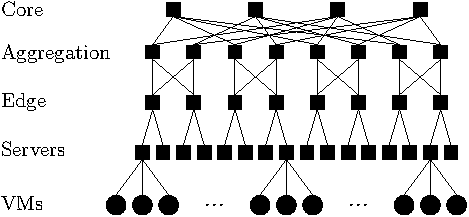
\includegraphics{figures/fat_tree-crop}
	\caption{An NFV enabled Fat Tree network topology with 4 ports and 3 VMs per server.}
	\label{fig:topology}
\end{figure}

A solution to a VNFPP specifies one or more paths through the network topology for each service. In particular, a path is a sequence of data center components that visit each VNF of a service in a prescribed order. Furthermore, each solution also specifies the amount of traffic that should be sent along each path.

The goal of the VNFPP is to provide a number of services by placing VNFs on VMs in the data center and defining the paths so as to maximize QoS and minimize capital and operational costs. In this paper, we formulate a three-objective VNFPP that takes two QoS metrics (i.e., latency and packet loss) and a cost metric (i.e., energy consumption) into account. An understanding of how the QoS and energy consumption interact is critical to the good operation of a data center. A multi-objective formulation of the VNFPP that considers how these metrics conflict informs the decision maker on the possible opportunities that are available. For example, a solver for a multi-objective formulation of the VNFPP enables the data center operator to:
\begin{itemize}
	\item Understand the cost-benefit trade off when increasing the amount of resources spent on services.
	\item Investigate how parameters such as network topology and the properties of servers and services could affect these trade offs.
	\item Make an informed selection from the set of possible trade off solutions.
\end{itemize}

%\begin{table}[t]
%	\caption{Lookup table of mathematical notations}
%	\label{tab:definition}
%	\center
%	\begin{tabular}{c|l}
%		\hline
%		Symbol & Definition \\
%		\hline
%        $\mathcal{S}$     & Set of all services \\
%        $\mathcal{C}$     & Set of all network components \\
%        $\mathcal{C}^{s}$ & Set of all servers \\
%        $\mathcal{V}$     & Set of all VNFs \\
%        $\mathcal{L}$     & Set of links connecting network components\\
%        $\mathcal{R}^s$   & Set of all routes for the service $s$ \\
%		$\mathcal{A}$     & Set of anti-affinity services \\
%		\hline
%		$\mathbb{P}^d_s$ & Service packet loss probability \\
%		$\mathbb{P}_{R^s_i}$ & The probability the route $R^s_{i}$ is taken \\
%		$\mathbb{P}^d_c$ & Component packet loss probability \\
%		$R^s_{i}$       & The $i$th route for service $s$ \\
%		$R^s_{i,j}$     & The $j$th component of the $i$th route of service $s$ \\
%		$W_s$ & Service latency \\
%		$\lambda_s$ & Service arrival rate \\
%		$\lambda_c$ & Component arrival rate \\
%		$\mu_c$ & Component service rate \\
%		$B_c$ & Component queue length $c$ \\
%		$\mathbb{W}_c$ & Component waiting time \\
%        \hline
%		$\gamma$ & Model threshold \\
%		$\Delta$ & Number of iterations below threshold \\ 
%
%		$N^M_v$ & Max number of instances of the VNF $v$ \\
%
%		$|\cdot|$ & Cardinality of a set or sequence \\
%		\hline
%	\end{tabular}
%\end{table}

\subsection{Mathematical Formulation}
\label{sec:formulation}

We first list some core terminologies important to the mathematical formulation of the objective and constraint functions of the VNFPP in this paper. $\mathcal{S}$ is the set of services that must be placed and $\mathcal{V}$ is the set of VNFs. A service $s=\{s_1,\cdots,s_n\}\in\mathcal{S}$ is a sequence of VNFs. The network topology is represented as a graph $\mathcal{G}=(\mathcal{C},\mathcal{L})$, where $\mathcal{C}$ denotes the set of data center components and $\mathcal{L}$ denotes the set of links connecting them. A route is a sequence of data center components where $\mathcal{R}^s$ is the set of paths for $s$, $R_{i}^s$ is the $i$th path of $s$ and $R_{i,j}^s$ is the $j$th component of this path. The complete notations are listed in Table I of Appendix A\footnote{The appendix document can be downloaded from \url{here}.}. %Finally, $|\cdot|$ indicates the cardinality of a set or a sequence. 

Overall, the VNFPP considered in this paper is defined as a MOP of the following three metrics.
\begin{itemize}
	\item The \textit{total energy consumption} (denoted as $E_C$).
	\item The \textit{mean latency} of the services (denoted as $L$):
	      \begin{equation}
		      L=\sum_{s\in\mathcal{S}} W_{s}/|\mathcal{S}|,
	      \end{equation}
	      where $W_s$ is the expected latency of $s\in\mathcal{S}$.
	\item The \textit{mean packet loss} of the services (denoted as $P$):
	      \begin{equation}
		      P=\sum_{s\in\mathcal{S}} \mathbb{P}^d_s/|\mathcal{S}|,
	      \end{equation}
	      where $\mathbb{P}^d_s$ is the packet loss probability of $s\in\mathcal{S}$.
\end{itemize}
In addition, there are five constraints associated with this VNFPP. Three of them are core constraints applicable to any VNFPP and are defined as follows.%The analytical modeling of these three metrics will be derived in~\pref{sec:system_model}.
\begin{itemize}
	\item Sequential data center components in a route must be connected by an edge:
	      \begin{equation}
		      (R_{i,j}^s, R_{i,j+1}^s) \in \mathcal{L}.
	      \end{equation}
	\item Each server can accommodate up to $N^V$ VNFs:
	      \begin{equation}
		      \sum_{v\in\mathcal{V}} A_v^{c_{\mathsf{s}}}<N^V,
	      \end{equation}
	      where $A_v^{c_{\mathsf{s}}}$ is the number of instances of the VNF $v$ assigned to the server ${c_{\mathsf{s}}}$.
	\item All VNFs must appear in the route and in the order defined by the service:
	      \begin{equation}
		      \pi^{R^s}_{s_i}\neq\emptyset,\quad\pi^{R_i}_{s_i}<\pi^{R_i}_{s_{i+1}},
	      \end{equation}
	      where $\pi^{R_i}_{s_i}$ is the index of the VNF $s_i$ in the route $R_i$.
\end{itemize}

In practice, security and legal concerns can impose additional constraints.
\begin{itemize}
	\setcounter{enumi}{3}
	\item A business may require an exclusive access to the servers in use due to security or performance restrictions. These requirements can be expressed through \textit{anti-affinity constraints} that restrict which services can share servers. For each service $s\in\mathcal{A}$ where $\mathcal{A}$ is the set of anti-affinity services, the anti-affinity constraints are defined as:
	      \begin{equation}
		      A^{c_{\mathsf{s}}}_{v_1}\cdot A^{c_{\mathsf{s}}}_{v_2}=0,\quad\forall v_1\in s, v_2\notin s.
	      \end{equation}

	\item VNFs may be provided under a license that restricts the number of instances of a VNF that can be created. These are known as the \textit{max instance constraints}:
	      \begin{equation}
		      \sum_{c_s\in\mathcal{C}^s} A_v^{c_{\mathsf{s}}}\leq N_v^M,
		      \label{eq:max_instances}
	      \end{equation}
	      where $N^M_v$ is the maximum number of instances of the VNF $v$ and $\mathcal{C}^{s}$ is the set of all servers.
\end{itemize}

The combination of the constraints and objectives results in a challenging optimization problem. Although each of the constraints can be considered independently, each constraint is complex such that the feasible search space is small relative to the overall search space. Further, the NP-Hardness of the problem means that the feasible search space still contains many solutions, few of which will be at or near optimal.

\subsection{Analysis of Feasible Search Space}
\label{sec:complexity}

It is acknowledged that VNFPP is a NP-hard problem~\cite{CohenLNR15,LuizelliCBG17,SangJGDY17} with various constraints. However, the relative size of the feasible region against the entire space has been overlooked in the literature. A small feasible region can make it significantly difficult to find feasible solutions, let alone optima.

In the context of VNFPP, a solution is feasible if at least one instance of every VNF has been placed. Here we plan to verify that the relative size of the feasible region, which is the probability of a randomly selected solution being feasible, is small. However, due to the NP-hardness of the VNFPP, there is no closed form solution of this relative size. Therefore, we estimate an upper bound instead. In particular, we consider the case where each VNF can be placed at any location independent of whether other VNFs have been placed therein. In the following paragraphs, we first verify that this is indeed an upper bound and then we provide a quantitative estimation to show that it is proportionately small.

\begin{lemma}
	The feasible region under the independence assumption is larger than the exact feasible region.\footnote{The proof can be found in the Appendix B.}
\end{lemma}

%\begin{proof}
%The independence assumption allows each VNF to be placed at any location independently of where other VNFs have been placed. We refer to the feasible region under the independence assumption as the independent feasible region. The independent feasible region contains all solutions where multiple VNFs occupy the same VM. In addition, it also contains all solutions where VNFs are not placed on the same location. This latter subspace is the exact feasible region and a subset of the independent feasible region.
%\end{proof}

Based on the independence assumption, the probability of a VNF being placed is calculated as:
\begin{equation}
	\mathbb{P}^p_{v}=1-\left(1-\frac{1}{|\mathcal{V}|}\right)^N,
\end{equation}
where $N$ is the number of VMs. Hence, the probability at least one VNF is not placed is calculated as:
\begin{equation}
	\mathbb{P}^{\neg p}=1-\left(\mathbb{P}^p_v\right)^{\mathcal{V}}.
\end{equation}
\pref{fig:p_feasible} plots the probability of generating a feasible solution for a data center with different capacities. From these trajectories, we find that the ratio of the feasible region against the entire search space approaches zero even for very low utilizations. The anti-affinity and max instance constraints further reduce the size of the feasible region, thus leading to a significantly increased difficulty.
\begin{figure}[t!]
	\centering
	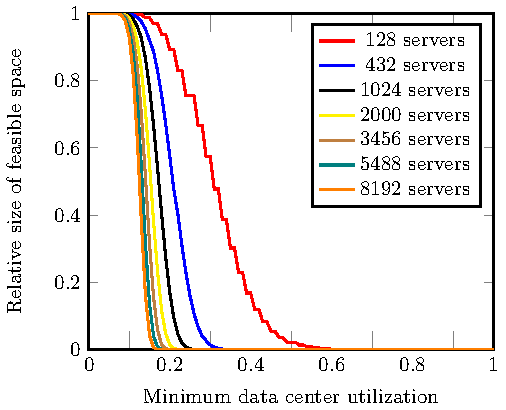
\includegraphics[width=\linewidth]{graphs/general/p_feasible}
	\caption{Demonstration of an upper bound of the proportion of the feasible region for different data center sizes. The proportionate size of the feasible region against the entire search space approaches zero even with a low utilization.}
	\label{fig:p_feasible}
	\vspace{1em}
\end{figure}

%In summary, the VNFPP is challenging not only because of its NP-hardness, but also its extremely small feasible region.


% !TeX root = ./main.tex
% ~ 3 pages

\section{System Model}
\label{sec:system_model}

In this section, we develop an analytical model to derive the three metrics that constitute the objective functions of our VNFPP given in~\pref{sec:problem_formulation}. They can be calculated for each service by examining the queues in the network. Each data center component consists of one or more buffers where packets are queued before being served. The arrival and service rates at a data center component determine the expected length of each queue, which in turn determine the waiting time and the probability of packet loss as well as the energy consumption. This information can then be used to calculate the latency, packet loss and energy consumption for each path of each service. In the following paragraphs, we first derive the approximation of the arrival rate for each data center component, based on which we calculate the three metrics. %considered in our VNFPP.

%\begin{algorithm}[t]
%	\KwData{Services $S$, service paths $R^s$, path selection probabilities $\mathbb{P}_{R^s}$, packet drop probabilities $\mathbb{P}^d_c$, service arrival rate $\lambda_s$}
%
%	\For{$s \in\mathcal{S}$} {
%		\For{$i \gets 0$ \KwTo $|\mathcal{R}^s|$} {
%
%			$\lambda \gets \lambda_{s} \cdot \mathbb{P}_{R^s_i}$ \tcp{Set route arrival rate}
%
%			\For{$c \in R^s_i$} {
%				$\lambda_{c} \gets \lambda_{c} + \lambda$ \tcp{Add rate to component}
%
%				$\lambda \gets \lambda \cdot (1 - \mathbb{P}_c^d)$ \tcp{Set departing rate}
%			}
%		}
%	}
%
%	\caption{Calculate the instantaneous expected arrival rates of all components}
%	\label{alg:calc_inst_arr}
%\end{algorithm}

\subsection{Arrival Rates of Data Center Components}
\label{sec:arrival_rate}

To calculate the arrival rate we must establish some reasonable assumptions about the system's behavior. In line with \cite{PoissonTraffic}, we assume the traffic generated by end users follows a Poisson distribution with a mean rate $\lambda_s$. As end users access the service independently, the total traffic arrival rate of a service can be calculated as the superposition of multiple independent Poisson processes. When packets arrive at a data center component, they are served with a first-in-first-out queueing strategy. To make the analytical model applicable to the practical implementation, instead of exploiting the infinite queueing strategies in \cite{InfiniteQueue}, we assume each data center component has a finite buffer length $B_c$. If the buffer becomes full, the newly arrived packets would be dropped to avoid system congestion. Finally, since packets are processed independently the time for a data center component to process a packet follows an exponential distribution with service rate $\mu_c$. Under these conditions, we model the service processing at each data center component as an M/M/1/B$_c$ system.

Next we can calculate the arrival rate of each data center component. Let $\lambda_c$ be the arrival rate of a data center component $c\in\mathcal{C}$. It is the sum of the packet flow rates of all paths entering this data center component. Due to the finite buffer size, the effective arrival rate $\lambda_c^e$ is less than the arrival rate and calculated as $\lambda _{ c }^{ e }=\lambda _{ c }{ \left( 1-\mathbb{P}^d_{c} \right)  }$, where $\mathbb{P}^d_{c}$ is the packet loss probability and is calculated as~\cite{Kleinrock75}:
\begin{equation}
    \mathbb{P}^d_{c}
	=
	\begin{cases}
		\frac{(1-\rho)\rho^{B_c}}{1-\rho^{B_c+1}}, & \text{if}\ \lambda\neq\mu\\
        \frac{1}{B_{c}+1}, & \text{otherwise}
	\end{cases},
	\label{eq:pl}
\end{equation}
where $\rho=\lambda_{c}/\mu_{c}$.

If the packet loss at a data center component were fixed then the arrival rate at each component would simply be the sum of the packet flow rates of the routes through that component. In practice, since the packet loss at a data center component depends on the arrival rate at the earlier components on the same path, dependency loops can form if the same component is visited multiple times in a sequence (as demonstrated in~\pref{fig:arrival_loop}). In this case, the packet loss probability at the revisited component becomes a function of its own arrival rate thus resulting in a dynamic system. Since the arrival rate at each component changes over time in a dynamic system, it is significantly more complex to derive the performance metrics based on the arrival rate. Existing works unfortunately neglect this factor by either considering models without packet loss (e.g., \cite{ZhangXLLGW17,QuZYSLR20,AgarwalMCD18}) or simply ignoring the dynamic feature of the system and only calculating the arrival rate at the outset instead (e.g.,~\cite{ChuaWZSH16,MarottaZDK17}). In this paper, we propose an iterative method to calculate the expected arrival rate over time. We first show that the arrival rates at all data center components naturally converge towards a fixed point given infinite time. Then, we elaborate the method that derives the expected arrival rate.

\begin{figure}[t!]
	\centering
	\begin{minipage}{0.24\textwidth}
		\centering
		\resizebox{0.9\textwidth}{!}{
			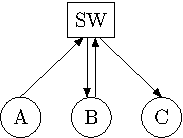
\includegraphics{figures/original_loop-crop}
		}
		\vspace{.2em}
		\subcaption{Original Configuration}
	\end{minipage}\hfill
	\vspace{2em}
	\begin{minipage}{0.24\textwidth}
		\centering
		\resizebox{0.9\textwidth}{!}{
			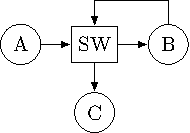
\includegraphics{figures/unfolded_loop-crop}
		}
		\vspace{.2em}
		\subcaption{Unfolded Loop}
	\end{minipage}

	\caption{Three VNFs (A, B, C) are visited in sequence through a single switch (SW). This forms a loop causing the arrival rate at the switch to be dependent on its own packet loss.}
	\label{fig:arrival_loop}
\end{figure}

\begin{lemma}
The arrival rate at each data center component converges towards a fixed point as time approach infinity.\footnote{The proof can be found in the Appendix B.}
\label{lemma:arrival_rate}
\end{lemma}

\begin{figure*}[t!]
	\centering
	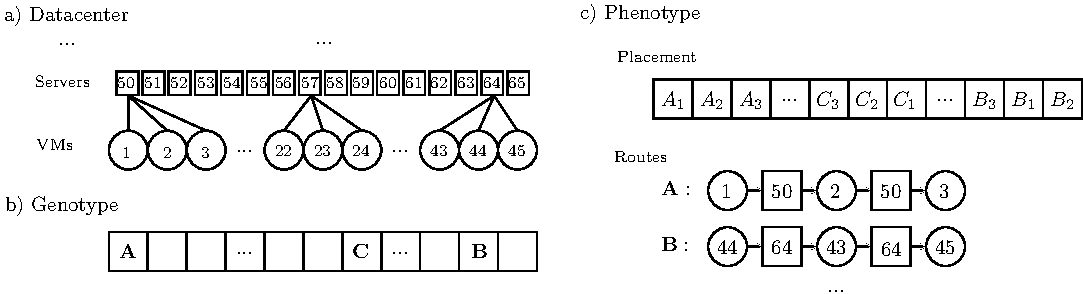
\includegraphics[width=\linewidth]{figures/solution_representation-crop}
	\caption{The genotype-phenotype solution representation used in this work.}
	\label{fig:gp_mapping}
\end{figure*}

%\begin{proof}
%Our proof considers a sequence of moments where the arrival rate is stable. We show that the instantaneous arrival rate $\lambda_t$ at any component at the time step $t$ is bounded by the arrival rates at the time steps $t-1$ and $t-2$. When $t\to\infty$, this bound converges towards a fixed value: %This is expressed as,
%\begin{equation}
%	\lim_{t\to\infty }{{\left|\lambda_{t-1}-\lambda_{t-2}\right|}}=0.
%\end{equation}
%%\noindent We show this by induction.
%
%Before carrying on our proof, we introduce the following two properties of the packet loss probability.
%\begin{itemize}
%	\item The packet loss probability strictly increases with the growth of arrival rate.
%	\item The packet loss probability asymptotically approaches $1$ with the growth of arrival rate.
%\end{itemize}
%
%Our proof is done by induction. We first prove that $\lambda_{t=2}$ is always bounded by $\lambda_{0}$ and $\lambda_{1}$ and then the inductive cases with $t\to \infty$. 
%
%When $t=0$, there is no packet in the queue, thus no packet is dropped. In this case, the effective arrival rate reaches its maximum. Furthermore, since the arrival rate is less than $\infty$ and the packet loss asymptotically approaches $1$, all future instances will have some packet lost where $\lambda_{t=0}>\lambda_{t>0}$. Since the effective arrival rate reaches its highest value at $t=0$, the packet loss probability at the next time step $\mathbb{P}^d_{t=1}$ must be the highest value. Hence, the effective arrival rate $\lambda_{t=1} < \lambda_{t>1}$. All in all, we have:
%\begin{equation}
%	\lambda_{t=1}<\lambda_{t=2}<\lambda_{t=0},
%\end{equation}
%where we denote $\lambda_{t=0}$ and $\lambda_{t=1}$ as the upper and lower bounds respectively.
%
%The inductive case consists of two parts.
%
%\begin{itemize}
%	\item We first show that if $\lambda_{t=n}$ is the lower bound of $\lambda$, then $\lambda_{t=n+1}$ will be the new upper bound. From the first property $\mathbb{P}^d_{t=n+1}<\mathbb{P}^d_{t=n}$, we have $\lambda_{t=n+1} > \lambda_{t=n}$. Furthermore, since $\lambda_{t=n} < \lambda_{t>n}$ and $\mathbb{P}^d_{t=n+1} < \mathbb{P}^d_{t>n+1}$, we have $\lambda_{t=n+1} > \lambda_{t>n}$ that makes $\lambda_{t=n+1}$ the new upper bound.
%	\item Secondly, we show that if $\lambda_{t=n}$ is the upper bound of $\lambda$, then $\lambda_{t=n+1}$ will be the new lower bound. From the first property $\mathbb{P}^d_{t=n+1} > \mathbb{P}^d_{t=n}$, we have $\lambda_{t=n+1}<\lambda_{t=n}$. Furthermore, since $\lambda_{t=n} > \lambda_{t>n}$ and $\mathbb{P}^d_{t=n+1}>\mathbb{P}^d_{t>n+1}$, we have $\lambda_{t=n+1}<\lambda_{t>n}$ that makes $\lambda_{t=n+1}$ the new lower bound.
%\end{itemize}
%
%Since the new upper and lower bounds of $\lambda$ are within the previous upper and lower bounds, they move towards each other at every time step and finally converge when $t\to \infty $.
%\end{proof}

A naive method of calculating the arrival rate, based on~\pref{lemma:arrival_rate}, is to evaluate the upper and lower bounds of the arrival rate until they converge. This is impractical since the theoretical result requires infinite time. Instead, this paper proposes to approximate the arrival rate by calculating the bounds until they converge to the point that further iterations are unlikely to change the expected arrival rate more than a threshold $\delta>0$. As the pseudo-code shown in Algorithm 2 in the Appendix C, it first initializes the packet loss at each data center component to 0 to simulate there being no packets in any queue (lines 3 to 4). In the main loop, the algorithm first calculates the current arrival rate and packet loss for each data center component by using the previous settings of packet loss (lines 6 to 8). From~\pref{lemma:arrival_rate}, we can see that the current arrival rate will be either a lower or upper bound of the arrival rate. Next the algorithm calculates the mean of the upper and lower bounds of the arrival rate for each data center component (line 12) and the divergence from the previous mean for each component (line 14). If the maximum divergence from the mean across all components has remained below $\delta$ for $\gamma>1$ iterations, future iterations are unlikely to alter the mean arrival rate. Hence, we terminate the process and output the mean arrival rate as the arrival rate at each data center component (lines 17 to 24).

Note that the parameters $\delta$ and $\gamma$ determine the accuracy and convergence speed of this model. A lower $\delta$ increases the model accuracy by requiring the mean to be more stable before being considered converged. The model is less sensitive to $\gamma$ which is required for the rare scenario where the bounds temporarily appear converged. We found that $\delta = 5.0$ and $\gamma = 10$ give a balanced trade-off between efficiency and accuracy. 

%\begin{algorithm}[t]
%	\KwData{Thresholds $\delta$ and $\gamma$}
%	\KwResult{Sets the arrival rate $\lambda_c$ for all components}
%	$N^i \gets 0$ \tcp{Sequential iterations below $\delta$}
%	
%	\For{$c \in C$}{
%		$\mathbb{P}^d_c \gets 0$ \tcp{Component packet loss}
%
%		$\overline{\lambda_c} \gets 0$ \tcp{Expected arrival rate}
%	}
%
%	Calculate $\lambda_c$ all components using \pref{alg:calc_inst_arr}
%	
%	\While{$N_{ci} < \gamma$}{
%
%		\For{$c \in C$}{
%			$\lambda^p_c \gets \lambda_c$  \tcp{Previous arrival rate of $c$}
%
%			Update $\mathbb{P}^d_c$ using $\lambda_c$ and \pref{eq:pl}
%		}
%
%		Update $\lambda_c$ of all components using \pref{alg:calc_inst_arr}
%
%		$M\!D \gets 0$ \tcp{Max. divergence}
%
%		\For{$c \in C$}{
%			\tcp{Calculate mean of current bounds}
%			$\overline{\lambda^p_c} \gets \left(\lambda^p_c + \lambda_c\right) /\ 2$
%
%			\tcp{Measure divergence of mean}
%			$D \gets \abs{\overline{\lambda^p_c} - \overline{\lambda_c}}$
%
%			\tcp{Update expected arrival rate}
%			$\overline{\lambda_c} \gets \overline{\lambda^p_c}$
%
%			\tcp{Update maximum divergence}
%			$M\!D \gets \textsc{Max}(D, M\!D)$
%		}
%
%		\eIf{$M\!D < \delta$}{
%			$N_{ci} \gets N + 1$
%		}{
%			$N_{ci} \gets 0$
%		}
%	}
%	
%	\tcp{Set final values of $\lambda_c$}
%	\For{$c \in C$}{
%		$\lambda_c \gets \overline{\lambda_c}$
%	}
%
%    % \Return $\lambda_c$
%	\caption{Calculate the stable expected arrival rates of all components}
%	\label{alg:calc_arr}
%\end{algorithm}

% However, if some loss of accuracy is permitted, we can closely approximate the fixed point by calculating the mean of the arrival rate over time until the change in the mean between time steps has remained less than a small amount $\delta$ for $\gamma$ iterations.

% \begin{lemma}
% The arrival rate calculation finishes in finite time if $\delta>0$ and $\gamma<\infty$.
% \end{lemma}

% \begin{proof}
% We prove this by showing any sequence of bound movements results in convergence. The bounds can either: 1) change by a small amount such that the mean does not change more than $\delta$, or 2) change by a large amount such that the \textit{does} change by more than $\delta$. In the first instance where there are $\gamma$ sequential small moves, the algorithm will terminate as the mean has changed by less than $\delta$ for $\gamma$ time steps. In the second instance, there are a finite number of large moves that can be performed before the bounds are too close for a large move to be possible and hence only small moves could occur. Likewise, any sequence of large and small moves must end with a sequence of small moves once the bounds are too close for a large move to be possible and only small moves can be applied. Since all possible actions end with a sequence of $\gamma$ sequential small moves, the algorithm must terminate in all instances.
% \end{proof}

% It would be possible for an `adversary' to prevent this calculation from being accurate by planning a sequence of $\delta$ small moves such that the algorithm terminates, followed by a single large move to introduce an error in the arrival rate calculation. This can only be avoided if $\delta=0$ and $\gamma=\infty$, in which case the process will not converge. However, in practice we find a low setting of $\gamma$ produces accurate results.

% Once the arrival rate has been determined the service latency, packet loss and datacenter energy consumption can then be calculated.

\subsection{Service Packet Loss}
\label{sec:packet_loss}

The packet loss probability of a service is the expected packet loss considering the probability of selecting each path:% It is calculated as:
\begin{equation}
    \mathbb{P}^d_s=\sum_{i=1}^{|\mathcal{R}^s|} \mathbb{P}^d_{R^s_i}\cdot \mathbb{P}_{R^s_i},
	\label{eq:pl_service}
\end{equation}
where $\mathbb{P}^d_{R^s_i}$ is the probability that a packet is dropped at any component on the path $R^s_i$. It is calculated as:
\begin{equation}
	\mathbb{P}^d_{R^s_i}=1-\prod_{c\in R^s_i}\left(1-\mathbb{P}^d_c\right).
	\label{eq:pl_path}
\end{equation}

\subsection{End-to-End Latency}
The end-to-end latency of a service is the expected waiting time over all paths. It is calculated as:
\begin{equation}
	W_s=\sum_{i=1}^{|\mathcal{R}^s|} W_{R^s_i} \cdot\mathbb{P}_{R^s_i},
\end{equation}

\noindent where $W_{R^s_i}$ is the average latency for $R^s_i$ and it is calculated as the sum of the waiting time at each data center component:
\begin{equation}
	W_{R^s_i} = \sum_{c\in R^s_i} W_c,
\end{equation}
where $W_c=\overline{N}/\hat{\lambda}_c$ is the waiting time at the component $c\in R^s_i$ and $\hat{\lambda}_c=\lambda_c\cdot\left(1-\mathbb{P}^d_c \right)$ is its effective arrival rate and $\overline{N}$ is its expected queue length~\cite{Kleinrock75}:
\begin{equation}
	\overline{N} = \begin{cases}
		\frac{\rho[1 - (B_c + 1)\rho^{B_c} + B_c\rho^{B_c+1}]}{(1 - \rho)(1 - \rho^{B_c+1})} , & \text{if } \ \lambda \neq \mu \\
		B_c/2,                                                                      & \text{otherwise}
	\end{cases}.
\end{equation}

\subsection{Energy Consumption}
\label{sec:energy}

The total energy consumption of a data center is the sum of energy consumed by each of its components. The energy consumption process follows a three-state model with \texttt{off}, \texttt{idle} and \texttt{active} states. Specifically, a component is \texttt{off} if its arrival rate is zero; it is \texttt{idle} while it is not processing any packet; otherwise, the component is \texttt{active}. A data center component does not consume any energy when it is \texttt{off}. Thus, we only need to consider the energy consumption of its \texttt{active} and \texttt{idle} states, denoted as $E^A$ and $E^I$, respectively. The total energy consumption of a data center is the sum of energy consumed by all its components:
\begin{equation}
    E_C=\sum_{c\in\mathcal{C}\setminus\mathcal{C}^{\mathsf{vm}}} U_c\cdot E^A+(1-U_c)\cdot E^I,
	\label{eq:sum_energy}
\end{equation}
where $\mathcal{C}^{\mathsf{vm}}$ is the set of VMs and $U_c$ is the utilization of the data center component $c$. To calculate $U_c$, we need to consider both single- and multiple-queue devices. The utilization of a queue is given by:
\begin{equation}
	\overline{U}_c =
	\begin{cases}
		0, & \rm{if} \ \lambda=0 \\
		\frac{1-\rho}{1-\rho^{B_c+1}}, & \rm{if}\ \lambda\le\mu \\ 
		\frac{1}{B_c+1}, & { \rm{otherwise} }
	\end{cases}.
	\label{eq:u}
\end{equation}
Physical switches can be modeled with a single-queue for their buffers. Hence the utilization of a switch $U_c$ is equal to the utilization of its queue:
\begin{equation}
    U_{c \in\mathcal{C}^{\mathsf{sw}}} = \overline{U}_c,
\end{equation}
where $\mathcal{C}^{\mathsf{sw}}$ is the set of switches. A server has multiple buffers: one for the virtual switch and one for each VNF. The server is \texttt{idle} when no packets are being processed at any of its buffers. Thus, the utilization of a server is calculated as:
\begin{equation}
	U_{c_{\mathsf{sr}}\in\mathcal{C}^\mathsf{sr}}=1-\left(1-\overline{U}_{c_{\mathsf{vs}}} \right)\cdot\prod_{c_{\mathsf{v}}\in\mathcal{A}^{c_{sr}}}\left(1-\overline{U}_{c_{\mathsf{v}}} \right),
	\label{eq:us}
\end{equation}
where $\mathcal{C}^\mathsf{sr}$ is the set of servers, $c_{\mathsf{vs}}$ is the virtual switch of the server and $\mathcal{A}^{c_\mathsf{sr}}$ is the set of VNFs assigned to the server $c_\mathsf{sr}$.


% !TeX root = ./main.tex

%\begin{algorithm}[t!]
%	
%	\KwData{Solution genotype $g$, total num. of VMs $N^T$, num. VMs per server $N^V$, set of services $S$}
%	\KwResult{Balanced solution $g$ modified in place}
%
%	$F \gets \emptyset$ \tcp{Set of free VMs}
%
%	$P \gets \emptyset$ \tcp{Set of used VMs}
%
%	\For{$s \in S$} {
%		$N^I_s \gets 0$ \tcp{Number of instances of service $s$}
%	}
%	
%	\tcc{\textbf{1. Find used/free VMs}}
%	\For{$i \gets 0$ \KwTo $N^T$} {
%		\eIf{$g_i = \texttt{None}$}{
%			\tcp{Record location of free VMs}
%			$F \gets F \cup i$
%		}{
%			\tcp{Record location of service instances}
%			$s \gets g_i$
%
%			$P \gets P \cup (i, s)$
%
%			$N^I_s \gets N^I_s + 1$
%		}
%	}
%	\tcc{\textbf{2. Find size of solution after mapping}}
%
%	$N^U \gets 0$ \tcp{Total num. VMs used after mapping}
%
%	\For{$s \in S$}{
%		$L_s \gets 0$ \tcp{Num. VMs used by the service}
%
%		\eIf{$s \in \mathcal{A}$}{
%			$L_s \gets \left\lceil \abs{s} / N^V \right\rceil \cdot N^V$
%		}{
%			$L_s \gets |S_i|$
%		}
%		$N^U \gets N^U + L_s \cdot N_s^I$
%	}
%	\tcc{\textbf{3. Assign missing services to free spaces}}
%	$M \gets \emptyset$ \tcp{Set of missing services}
%	\For{$s \in S$}{
%		\If{$N^I_s = 0$}{
%			$M \gets M \cup s$
%		}
%	}
%
%	\While{$\abs{M} > 0 $ and $ \abs{F} > 0$}{
%		$i \gets \text{\textbf{pop} first free VM from} \; F$
%
%		$s \gets \text{\textbf{pop} first missing service from} \; M$
%
%		$g_i \gets s$ \tcp{Assign service to VM}
%
%		$N^U \gets N^U + L_s$
%	}
%
%	\tcc{\textbf{4. Swap service instances until feasible}}
%
%	\textbf{Sort} service instances in $P$ by their contribution (\pref{eq:contribution}) in ascending order
%
%	\While{$N^U > N^T$ or $\abs{M} > 0$} {
%		$(i, s) \gets $ \textbf{pop} first service instance in $P$
%
%		$g_i \gets \texttt{None}$ \tcp{Free VM}
%
%		$N^U \gets N^U - L_s$
%
%		\If{$\abs{M} > 0$}{
%			$s \gets \textbf{pop } \text{first missing service from } M$ 
%
%			$g_i \gets s$
%
%			$N^U \gets N^U + L_s$
%		}
%	}
%	\caption{Balances the number of instances of each service to ensure feasibility.}
%	\label{alg:balance}
%\end{algorithm}

\section{Proposed Evolutionary Optimization Framework for VNFPPs}
\label{sec:optimisation}

In this section, we propose a tailored evolutionary optimization framework to solve the three-objective VNFPP defined in~\pref{sec:problem_formulation}. There are two tailored features: one is a genotype-phenotype solution representation, detailed in~\pref{sec:representation}, that guarantees feasible solutions for the underlying VNFPP; the other is a tailored initialization operator, detailed in~\pref{sec:operators}, built upon the solution representation to produce a good initial population. Note that these tailored features can be readily incorporated into any existing EMO algorithm as shown in~\pref{sec:incorporation}. Although these operators are specifically designed for the Fat Tree network topology~\cite{AlFaresLV08} (see~\pref{fig:topology}) given its wide adoption in industry~\cite{LebiednikMT16}, we argue that our model and problem formulation are generally useful for any network topology.

\subsection{Genotype-Phenotype Solution Representation}
\label{sec:representation}
%A poor solution representation largely leads to an ineffective search process. 
\textcolor{red}{One of the key challenges when designing and/or applying EAs to real-world optimization problems is how to encode the problem into a solution in EA. In this paper, we propose a genotype-phenotype solution representation for our VNFPP. As shown in \pref{fig:gp_mapping}, the genotype is a string of characters where each character can be either a service $s\in S$ or a sentinel \texttt{NONE}, i.e., the corresponding VM is not in use (illustrated in the figure with an empty character). The phenotype is a set of paths and the corresponding path probabilities required for the VNFPP. The mapping between them defines how to transform the genotype into the corresponding phenotype. Due to the existence of complex constraints defined in~\pref{sec:problem_formulation}, a simple mapping does not always lead to a feasible solution. The main crux of our genotype-phenotype solution representation is the use of problem-specific heuristics at the mapping stage that avoid generating infeasible solutions. It consists of three steps: \texttt{balance}, \texttt{placement} and \texttt{routing}.}

\begin{figure*}[t!]
	\begin{subfigure}[T]{.3\linewidth}
		\centering
		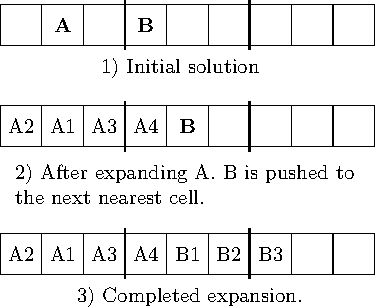
\includegraphics[width=\columnwidth]{figures/simple_expansion-crop}
		\caption{Simple expansion.}
		\label{fig:1a}
	\end{subfigure}\hfil
	\begin{subfigure}[T]{.3\linewidth}
		\centering
		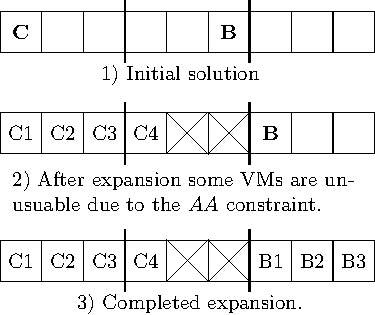
\includegraphics[width=\columnwidth]{figures/aa_expansion-crop}
		\caption{Anti-affinity expansion.}
		\label{fig:1b}
	\end{subfigure}\hfil
	\begin{subfigure}[T]{.3\linewidth}
		\centering
		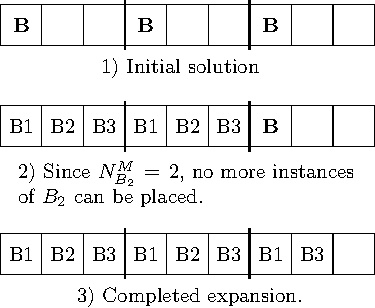
\includegraphics[width=\columnwidth]{figures/limited_expansion-crop}
		\caption{Max instances expansion}
		\label{fig:1c}
	\end{subfigure}
	\vspace{2em}
	\caption{This figures shows three examples of the placement step of the genotype-phenotype mapping. There are three services here: service $\mathbf{A} = \{ A_1, A_2, A_3, A_4\}$ , service $\mathbf{B} = \{B_1, B_2, B_3\}$ which has a max instances constraint $N_{B_2}^M = 2$ and service $\mathbf{C} = \{C_1, C_2, C_3, C_4\}$. In addition, $\mathcal{A} = \{C\}$ such that service $\mathbf{C}$ cannot share a server with any other service. Tall lines indicate server boundaries.}
	\label{fig:placement}
\end{figure*}


\subsubsection{Balance}

The \texttt{balance} step adds and/or removes service instances to guarantee the feasibility after the genotype-phenotype mapping. This is implemented by ensuring that the genotype has at least one instance of each service and the total number of VMs being used does not exceed the available number in the data center. The pseudo-code is given in Algorithm 3 in Appendix C. It first identifies the location of all unused VMs along with the location and number of each service instance (lines 6 to 14). Using this information, the algorithm can calculate the number of VMs the solution will require after the mapping (lines 16 to 23) and identify missing services that have no service instances (lines 24 to 28). The algorithm then places a service instance for any missing services on a free VM if possible (lines 29 to 33). Finally, if there is insufficient space to place a missing service instance or the expanded length of the solution would exceed the total capacity, the algorithm removes the service instance with the lowest contribution and, if necessary, replaces it with a service instance for a missing one (lines 35 to 43). In particular, the contribution of an instance is evaluated as the change in the service instance utilization if it were removed:
\begin{equation}
	C^s_i = \frac{\lambda_{s}}{\mu_{s_1} \cdot (i - 1)} - \frac{\lambda_{s}}{\mu_{s_1} \cdot i},
	\label{eq:contribution}
\end{equation}
\noindent where $C^s_i$ is the contribution of the $i$th instance of $s$ and $\mu_{s_1}$ is its service rate of the first VNF. As the arrival rate is distributed over each VNF, a service with several instances will have some instances with a low contribution. On the other hand, if a service has only one instance, it will have an infinite contribution. This minimizes the impact on the service quality when removing solutions. 

\subsubsection{Placement}

The \texttt{placement} step uses a first feasible heuristic, a variant of the first fit heuristic from the cloud computing literature~\cite{KellerTLB12}, to place the VNFs of a service in the phenotype close to the position of the service instance in the genotype without violating any constraint. The first feasible heuristic is executed on each service instance. It places the first VNF of the service on the nearest VM to the service instance that would not result in a constraint violation. This is repeated from the new position for the next VNF instance until all VNFs are placed. As anti-affinity services reserve the whole of a server, they must be placed first to ensure the service is not fragmented across multiple servers and does not reserve more space than necessary. \pref{fig:placement} presents three examples of the \texttt{placement} step for different scenarios.

\subsubsection{Routing}

Finally, the \texttt{routing} step finds the set of shortest paths between the VNFs of each service instance to complete a solution. A Fat Tree network can be efficiently traversed by stepping upwards to the parent switch until a common ancestor between the initial and the target VNFs is found. In the Fat Tree network topology, there can be several routes between VNFs sharing the same distance. In this paper, we apply the equal-cost multi-path routing strategy~\cite{Hopps2000} to distribute the traffic evenly over all shortest paths between sequential VNFs. This strategy has been shown to be optimal for Clos data center networks such as the Fat Tree~\cite{ChiesaKS17}.

\subsection{Tailored Initialization Operator}
\label{sec:operators}

In this paper, we propose a tailored initialization operator adapted to the characteristics of VNFPP and thus boost an effective exploration of the search space.

The goal of initialization is to generate a set of diverse initial solutions to \lq jump start\rq\ the search process afterwards. Note that both the placement and the number of instances in the VNFPP can influence the solution quality. Uniform sampling, one of the most popular initialization strategies, varies the placement of service instances but the expected number of instances remains the same across all solutions. To amend this problem, we propose a variant of uniform sampling where service instances are placed uniformly at random, but the number of instances of each service varies across the population. More specifically, we first calculate the maximum number of instances of each service that can be accommodated in a data center. Thereafter, the solution is initialized by placing some fraction of this number of instances of each service. For the $i$th solution, the number of instances of the service $s$ is calculated as:
\begin{equation}
	N^I_{i,s} = \left\lfloor \frac{i}{N} \cdot \frac{N}{\sum_{s\in S} \abs{s}} \right\rfloor,
	\label{eq:num_services}
\end{equation}
where $N$ is the population size. For example, if the population size $N=100$, the $100$th solution will have twice as many instances of each service as the $50$th solution.

% \subsubsection{Mutation Operators}

% The mutation operators should aid in producing diverse solutions so as to have an appropriate exploration of the search space. Since both the number and the position of the VNF instances is important, we define two mutation operators, dubbed as \texttt{swap} and \texttt{add/delete}, each of which can be applied on a VM according to the mutation rate. More specifically:
% \begin{itemize}
%     \item The \texttt{swap} operator exchanges the contents two VMs. This operator aims to promote horizontal movement of service placements.
% 	\item The \texttt{add/delete} operator removes a service instance if it exists; otherwise it adds a randomly selected service. This operator helps to optimize the number of service instances.
% \end{itemize}
% When mutation occurs one of the operators are selected with equal probability. \pref{fig:mutation} uses two illustrative examples to further explain the working mechanisms of these operators.

% \begin{figure}[t]
% 	\centering
% 	\begin{subfigure}[T]{\linewidth}
% 		\centering
% 		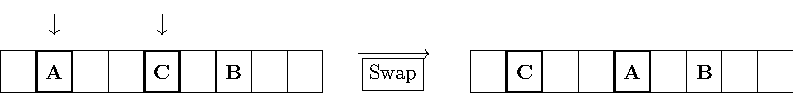
\includegraphics[width=\columnwidth]{figures/swap}
% 		\caption{The \texttt{swap} operator exchanges two randomly selected VMs.}
% 		\label{fig:swap}
% 	\end{subfigure}

% 	\vspace{1.5em}

% 	\begin{subfigure}[T]{\linewidth}
% 		\centering
% 		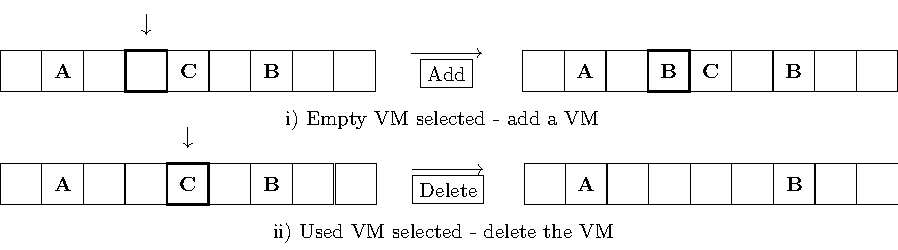
\includegraphics[width=\columnwidth]{figures/add_remove}
% 		\caption{The \texttt{add/delete} operator selects a VM and adds a VM if it is not in use or removes one otherwise.}
% 		\label{fig:add_remove}
% 	\end{subfigure}
% 	\vspace{1em}
% 	\caption{Illustrative examples of the \texttt{swap} and \texttt{add/delete} operators.}
% 	\label{fig:mutation}
% \end{figure}

\subsection{Incorporation into EMO Algorithms}
\label{sec:incorporation}

The solution representation and initialization operators proposed in~\pref{sec:representation} and~\pref{sec:operators} can be incorporated into any EMO algorithm. In this paper, we integrate it into NSGA-II~\cite{DebAPM02} as a proof of concept. It is worth noting that we do not need to make any modification on the environmental selection of the baseline algorithm. \textcolor{red}{Further, we found the classic uniform crossover and mutation reproduction operators to be sufficient to vary and exchange information on the number and position of service instances.}


% ~ 1 page
% !TeX root = ./main.tex

\section{Empirical Study}
\label{sec:experiments}
We seek to answer the following six research questions (RQs) through our experimental evaluations.
\begin{itemize}
    \item\underline{\textbf{RQ1}}: How accurate is the QoS model developed in~\pref{sec:system_model} compared to others in the literature?
    \item\underline{\textbf{RQ2}}: How do different EMO frameworks compare on the VNFPP?
    \item\underline{\textbf{RQ3}}: Is an accurate QoS model beneficial compared to surrogate models used in the literature?
    \item\underline{\textbf{RQ4}}: Does the proposed solution representation improve upon alternative solution representations?
    \item\underline{\textbf{RQ5}}: How does the tailored EMO algorithm compare against the state-of-the-art peers?
    \item\underline{\textbf{RQ6}}: How well do the proposed operators cope with challenging constraints in VNFPP?
\end{itemize}

%\begin{table}[t]
%    \vspace{1em}
%    \centering
%    
%    \caption{Parameter settings used in evaluation}
%    \label{tab:parameter}
%    \begin{tabular}{ll}
%        \toprule
%        Parameter                             & Setting        \\
%        \midrule
%        Mean service arrival rate             & 10 requests/ms \\
%        Variance service arrival rate         & 3 requests/ms  \\
%        \midrule
%        Per port service rate                 & 20 requests/ms \\
%        Per port queue length                 & 20 requests    \\
%        Server active energy cost             & 30 kw/h        \\
%        Server idle energy cost               & 10 kw/h        \\
%        \midrule
%        Min. data center utilization          & 60\%           \\
%        Mean service length                   & 5 VNFs         \\
%        Variance service length               & 1 VNFs         \\
%        Min service length                    & 2 VNFs         \\
%        \midrule
%        Mean VNF service rate                 & 10 requests/ms \\
%        Variance VNF service rate             & 3 requests/ms  \\
%        VNF queue length                      & 20             \\
%        \midrule
%        Model tolerance $\left(\delta\right)$ & 5.0            \\
%        Min. iterations $\left(\gamma\right)$ & 10             \\
%        \midrule
%        Population size $\left(n\right)$      & 120            \\
%        Mutation rate                         & 1/$n$          \\
%        Crossover probability                 & 0.9            \\
%        Number of evaluations                 & 1200           \\
%        \bottomrule
%    \end{tabular}
%\end{table}

\subsection{Parameter settings}
The parameter settings used in this work are listed in Table II in the Appendix D. To reflect the mechanism of real switches, the service rate and queue length of each switch in our model are the sum of the service rates and queue lengths of each port. For example, a switch with $8$ ports will have a service rate of $8\times 20=160$ requests/ms. To create a VNFPP instance, we generate enough services to hit the target minimum data center utilization. For example, if the data center has $1,000$ VMs, the expected service length is $5$ and the target data center utilization is $50$\%, then there will be $100$ distinct services. Next, the service arrival rate and length and the VNF service rate are set for each service and VNF by sampling from a Gaussian distribution with the means and variances specified in Table II in the Appendix D.

\subsection{Evaluation of QoS Model Accuracy}
\label{sec:model_accuracy}

\subsubsection{Methods}
The QoS model developed in~\pref{sec:system_model} stands for the foundation of this study. Its correctness and accuracy determine whether our algorithm is applicable to real-world problems. To answer RQ1, we evaluate the accuracy of the model by comparing its predictions against benchmark measurements taken from a simulated data center.

\textcolor{red}{To create the benchmark, we generate $100$ VNFPP problems for a data center with $412$ servers to constitute a diverse set of problems. Then, we use our proposed initialization operator (see \pref{sec:operators}) to generate $100$ candidate solutions for each problem.} Next, we evaluate each solution by using our proposed model and select four solutions for evaluation: 1) the one with the lowest latency; 2) the one with the lowest packet loss; 3) the one with the lowest energy consumption; and 4) the one that best balances all objectives. By using diverse solutions, we can rule out any inaccuracy reflected by the model. For example, if the model is poor at predicting the latency, the data set will contain a solution with a high expected latency that highlights this issue. %As simulation is slow we are only able to evaluate a select number of solutions. 

To get accurate measurements for the benchmark, we apply a discrete event simulator (DES) to calculate each metric of a solution. A DES simulates the transmission of each packet through the data center to produce accurate measurements of the QoS and energy consumption. In our experiments, the DES is based on the same assumptions introduced in \pref{sec:system_model} and it is used to evaluate each solution for a range of arrival rates.

We compare our model against two other accurate models used in the literature.%: an M/M/1 queueing model and an M/M/1/B$_c$ queueing model.
\begin{itemize}
    \item \underline{M/M/1 queueing model}: As one of most popular models in the literature~\cite{PeiHXLWW20,JemaaPP16,BaumgartnerRB15}, it models the data center as a network of queues and assumes that each queue has an infinite length. Under this assumption, there is no packet loss. However, if the arrival rate at a queue is greater than or equal to its service rate, the length of the queue will tend towards infinity that leads the waiting time to approach infinity and the utilization to approach $100$\%.
    \item \underline{M/M/1/B$_c$ queuing model}: In contrast, this model consider queues with a finite length. Existing M/M/1/B$_c$ queueing models like~\cite{ChuaWZSH16} consider packet loss but not feedback loops. In essence, they calculate the instantaneous arrival rate and packet loss at each data center component when the services are first started.
\end{itemize}

\subsubsection{Results}
\pref{fig:model_sim} shows the estimates of each metric by different models benchmarked against the ground-truth measurements. The closer the model matches the benchmark, the more accurate the model is. From the results, we find that our proposed model is significantly more accurate than the other peer queueing models. This reflects how our model correctly captures the impact of feedback loops on the QoS and energy consumption.

In contrast, the M/M/1/B$_c$ queueing model, which does not account for feedback loops, is overly pessimistic with a high latency, packet loss and energy consumption. This is because the M/M/1/B$_c$ model calculates the instantaneous arrival rate at the start of operation. As shown in Lemma \ref{lemma:arrival_rate}, this is always higher than the arrival rate after convergence.

Likewise, these results also demonstrate the drawbacks of the commonly used M/M/1 model. First, the model falsely assumes that the queue at a component can grow to an infinite length and as a consequence believes that packet loss is zero in all situations. As a result, the model becomes less reliable as the arrival rate increases and packet loss becomes large.

\vspace{0.5em}
\noindent
\framebox{\parbox{\dimexpr\linewidth-2\fboxsep-2\fboxrule}{
        \textbf{\underline{Response to RQ1:}} \textit{Due to an understanding of the impact of feedback loops, our proposed model gives significantly more accurate estimates of the QoS and energy consumption than other models when packet loss is considered.}
    }}

\begin{figure*}[t!]
    \centering
    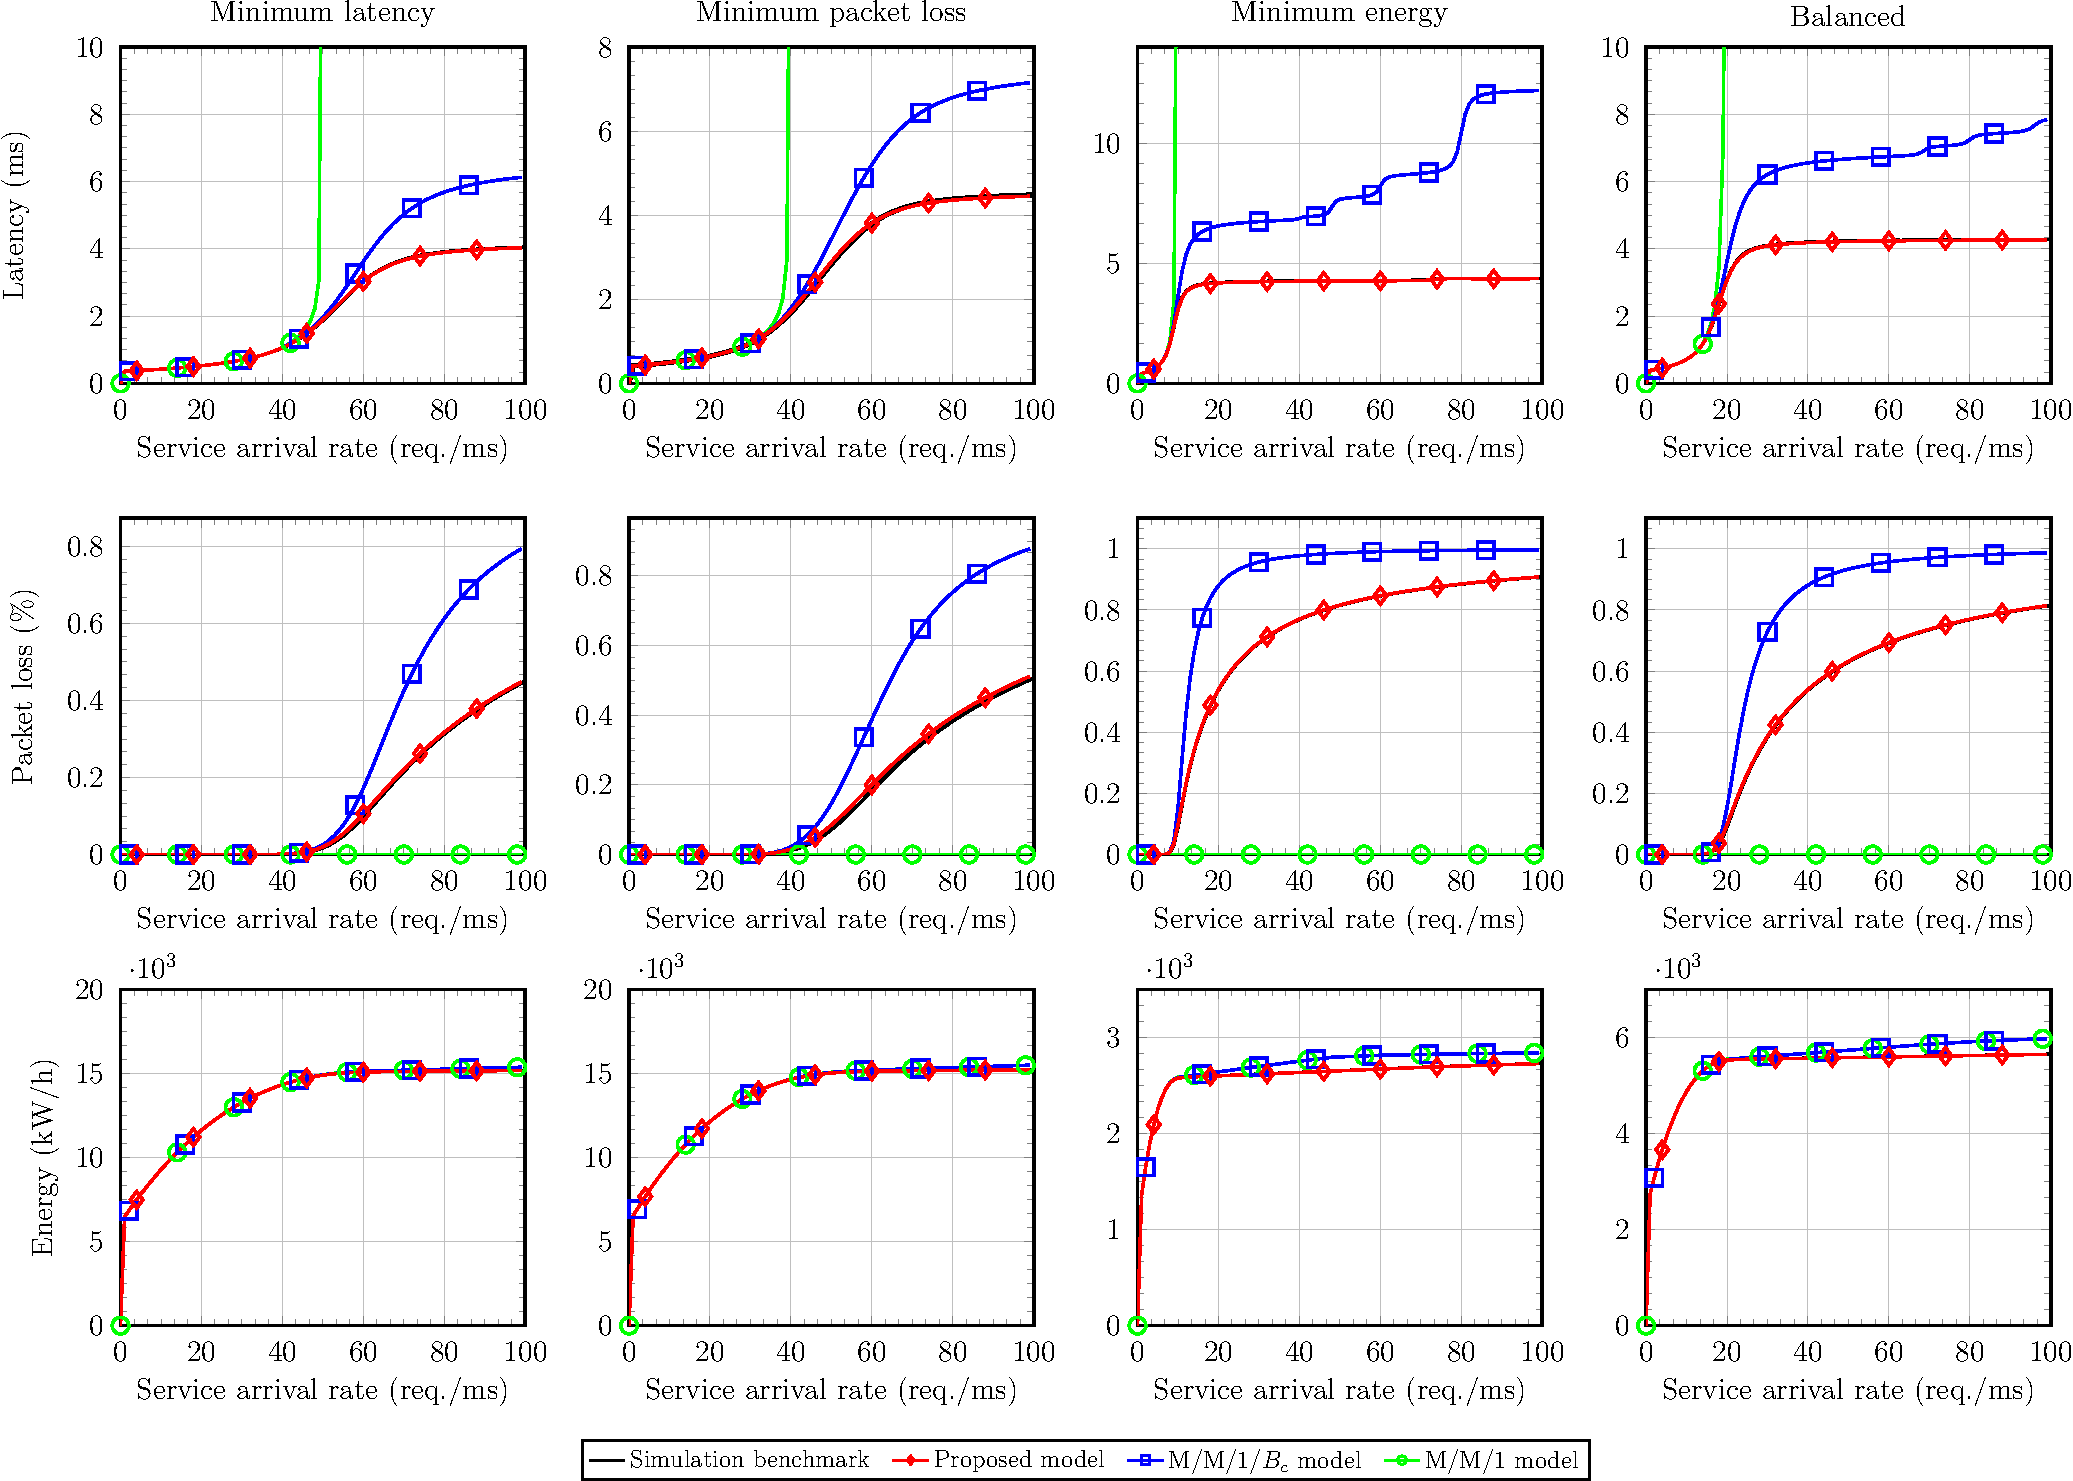
\includegraphics[width=\linewidth]{graphs/general/model_sim-crop}
    \caption{Comparison results of three different metrics estimated by our proposed model against the other two queueing models.}
    \label{fig:model_sim}
\end{figure*}

\subsection{Comparison with Other MOEA Frameworks}
\label{sec:moea_comparison}

\subsubsection{Methods}
\textcolor{red}{To illustrate that our operators can be integrated into any MOEA framework, we compare the quality of solutions obtained when different MOEAs are used with our proposed operators. Specifically, we integrated our proposed operators into three state of the art MOEAs: NSGA-II \cite{DebAPM02}, MOEA/D \cite{ZhangL07} and IBEA \cite{ZitzlerK04}.}

\textcolor{red}{
In our experiments, we generate $30$ VNFPP instances for six data centers with different sizes. To compare the performance of different algorithms, we use the QoS model developed in~\pref{sec:system_model} to evaluate the objective functions of the solutions obtained by different algorithms and use the HV indicator as the performance measure.
}

\textcolor{red}{
\subsubsection{Results}
The results of this test are illustrated in~\pref{fig:moea_comparison}. We found that all algorithm performed similarly, with no algorithm performing consistently significantly better than any other. Given all algorithms performed similarly, we have selected NSGA-II for use in future tests based on its widespread adoption in the literature. 
}

\begin{figure}[t!]
    \centering
    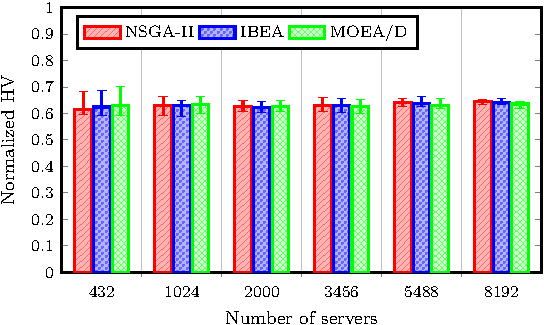
\includegraphics[width=\linewidth]{graphs/moeas/comparison-crop}
    \caption{Inter-quartile range of the HV for different MOEAs.}
    \label{fig:moea_comparison}
\end{figure}

\vspace{0.5em}
\noindent
\framebox{\parbox{\dimexpr\linewidth-2\fboxsep-2\fboxrule}{
    \textcolor{red}{\textbf{\underline{Response to RQ2:}} \textit{From our empirical results, we find that all MOEAs using our proposed operators performed comparably.}
    }}}

\subsection{Benefit of Queueing Models}
\label{sec:model_benefit}

\subsubsection{Methods}
% \! is to fix the odd space that \cite introduces after the bracket

To answer RQ3, we compare the quality of solutions obtained by our tailored EMO algorithm when using different QoS models including three queueing models studied in~\pref{sec:model_accuracy} and three popular surrogate models briefly introduced as follows.
\begin{itemize}
    % Explain the reasoning behind these surrogates
    \item\underline{Constant waiting time or packet loss (CWTPL)}: As in~\cite{HawiloJS19} and~\cite{VizarretaCMMK17}, this model assumes that the waiting time at each data center component is a constant. In addition, we also keeps the packet loss probability at each component as a constant. Based on these assumptions, we can evaluate the latency and packet loss for each service and apply the metric of the energy consumption developed in~\pref{sec:energy}. All these constitute a three-objective problem that aims to minimize the average latency, packet loss and total energy consumption.

    \item\underline{Resource utilization (RU)}: As in~\cite{ChantreF20,QiSW19} and~\cite{GuoWLQA0Y20}, this model assumes that the waiting time is a function of the CPU demand and the CPU capacity of each VM. In addition, the demand is assumed to determine the packet loss probability as well. Based on these assumptions, we evaluate the latency for each service and apply the metric of the energy consumption developed in~\pref{sec:energy}. All these constitute a two-objective problem that aims to minimize the average latency (and by extension the packet loss) and the total energy consumption.

    \item\underline{Path length and used servers (PLUS)}: This model uses the percentage of used servers to measure the energy consumption (e.g.,~\cite{MiottoLCG19,RankothgeLRL17,LiuZDLGZ18}) and the length of routes for each service as a measure of service latency, packet loss or quality (e.g.,~\cite{LuizelliCBG17,AllegKMA17,BeckB15}). All these constitute a two-objective problem that aims to minimize the path length and the number of used servers.
\end{itemize}

In our experiments, we generate $30$ problem instances of the Fat Tree data center with $432$, $1,024$, $2,000$, $3,456$, $5,488$ and $8,192$ servers respectively. At the end, the non-dominated solutions found by our tailored EMO algorithm with different QoS models are re-evaluated by using the QoS model developed in~\pref{sec:system_model}. The quality of these non-dominated solutions is evaluated by the Hypervolume (HV) indicator~\cite{ZitzlerT99} that measures both the convergence and diversity of the population, simultaneously.

\subsubsection{Results}

From the results shown in Figs.~\ref{fig:model_objectives} and~\ref{fig:model_benefits}, we find that the solutions obtained by using our proposed model and the M/M/1/B$_c$ queueing model are comparable with each other while they are significantly better than those obtained by using other models in terms of the population diversity.

%\pref{fig:model_benefits} shows that the choice of model had a significant impact on the quality and diversity of the solutions in the final population. The populations proposed by our model and the M/M/1/$B_c$ model are more diverse than the alternative models and typically have lower average latency, packet loss and energy consumption. Notably, neither of the models produce significantly better ($p < 0.05$) populations than the other as measured by the HV and a Wilcoxon Rank Sum test \cite{ArcuriB11}. This is despite the M/M/1/$B_c$ model giving less accurate measurements of the metrics. Clearly, strict parity with the simulation is not essential for the algorithm to find good solutions but only that the simulation and model agree on the ordering of solutions, i.e. given any two solutions $x$ and $y$, both models will agree whether $x$ is better, worse or equivalent to $y$ in each objective. From these results and \pref{fig:model_sim}, it seems likely that M/M/1/$B_c$ and our proposed model meet this criteria.

Specifically, populations obtained with the M/M/1 queueing model have poor diversity. This can be attributed to the inability of the M/M/1 queueing model to distinguish solutions by the latency or packet loss metrics. In particular, most solutions obtained by using the M/M/1 queueing model have an infinite latency and no packet loss. This is because if the arrival rate at any data center component is larger than the service rate, the waiting time at that component tends towards infinity. Hence the average latency also tends towards infinity. As all solutions have the same latency and packet loss, the optimization algorithm can only distinguish solutions based on their energy consumption. As a result, only solutions with low energy consumption survive.

For a similar reason, the surrogate models also failed to produce diverse solutions. Despite their differences, none of the surrogate models provide any incentive to vary the number of service instances. For example, both the CWTPL and PLUS models benefit from shorter average routes. However, increasing the number of service instances will also increase the number of servers yet is unlikely to decrease the average service length. Likewise, for the RU model, increasing the number of service instances increases the energy consumption and makes it more difficult for the algorithm to find servers with a low resource utilization.

\begin{figure}[t!]
    \centering
    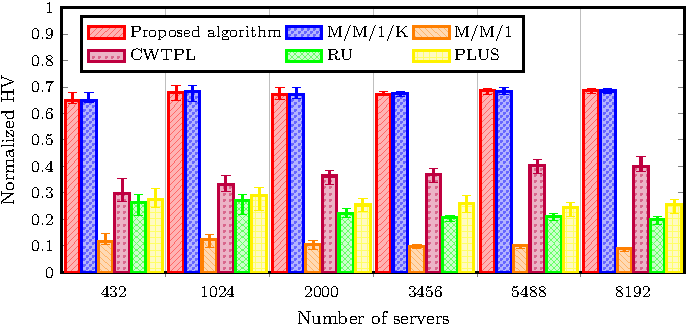
\includegraphics[width=\columnwidth]{graphs/model/models-crop}
    \caption{Inter-quartile range of the HV when using different surrogate models as the objective function.}
    \label{fig:model_benefits}
\end{figure}

\vspace{0.5em}
\noindent
\framebox{\parbox{\dimexpr\linewidth-2\fboxsep-2\fboxrule}{
        \textbf{\underline{Response to RQ3:}} \textit{The queueing models that account for the packet loss lead to significantly more diverse solutions compared to the other queueing model(s) as well as the surrogate models.}
    }}
\textcolor{red}{
\subsection{Evaluation of Solution Representation}
\label{sec:alternative_representations}
}
\textcolor{red}{To answer RQ4, we compare the quality of solutions obtained when different solution representations are applied to the VNFPP. Specifically, the following two meta-heuristic algorithms use NSGA-II as the baseline but have different solution representations.
\begin{itemize}
    \item\underline{Binary representation}: As in \cite{ChantreF20,KaurGK020,CharismiadisTPM20}, a string of binary digits are used to represent if a VNF is assigned to a server.
    \item\underline{Direct representation}: As in \cite{RankothgeLRL17}, a solution is directly represented as a string of VNFs.
\end{itemize}
In our experiments, we generate $30$ VNFPP instances for six data centers with different sizes. To compare the performance of different algorithms, we use the QoS model developed in~\pref{sec:system_model} to evaluate the objective functions of the solutions obtained by different algorithms and use the HV indicator as the performance measure.}

\begin{figure}[t!]
    \centering

    \begin{subfigure}[b]{0.48\linewidth}
        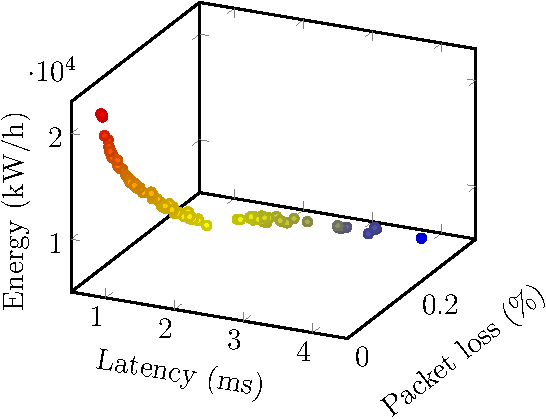
\includegraphics[width=\textwidth]{graphs/model/proposed-crop}
        \caption{Proposed}
    \end{subfigure}
    \begin{subfigure}[b]{0.48\linewidth}
        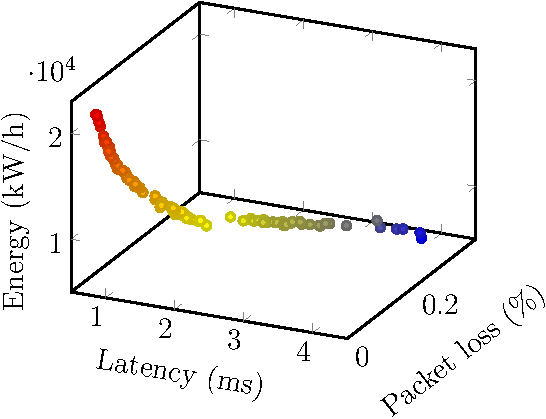
\includegraphics[width=\textwidth]{graphs/model/mm1k-crop}
        \caption{M/M/1/$B_c$}
    \end{subfigure}

    \vspace{1em}

    \begin{subfigure}[b]{0.48\linewidth}
        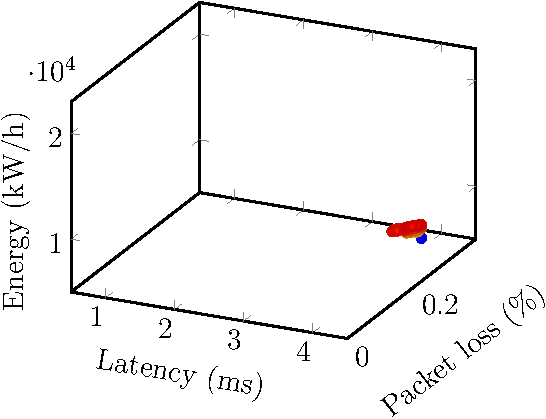
\includegraphics[width=\textwidth]{graphs/model/mm1-crop}
        \caption{M/M/1}
    \end{subfigure}
    \begin{subfigure}[b]{0.48\linewidth}
        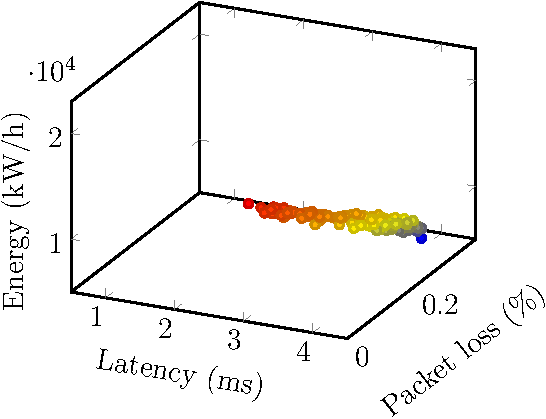
\includegraphics[width=\textwidth]{graphs/model/constant_energy-crop}
        \caption{CWTPL}
    \end{subfigure}

    \vspace{1em}

    \begin{subfigure}[b]{0.48\linewidth}
        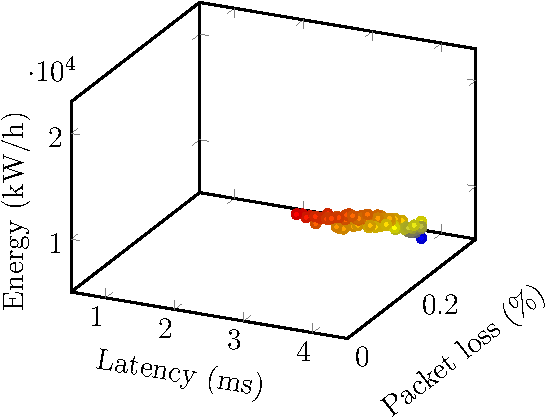
\includegraphics[width=\textwidth]{graphs/model/resources_energy-crop}
        \caption{RU}
    \end{subfigure}
    \begin{subfigure}[b]{0.48\linewidth}
        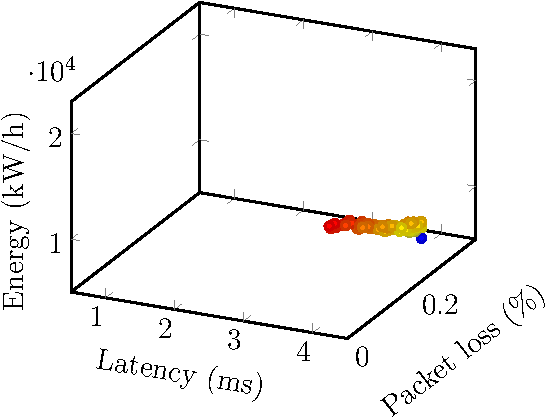
\includegraphics[width=\textwidth]{graphs/model/length_used-crop}
        \caption{PLUS}
    \end{subfigure}
    \vspace{1em}
    \caption{\textcolor{red}{Non-dominated front found by our algorithm when different models are used as the objective function.}}
    \label{fig:model_objectives}
\end{figure}

\begin{figure}[t!]
    \centering
    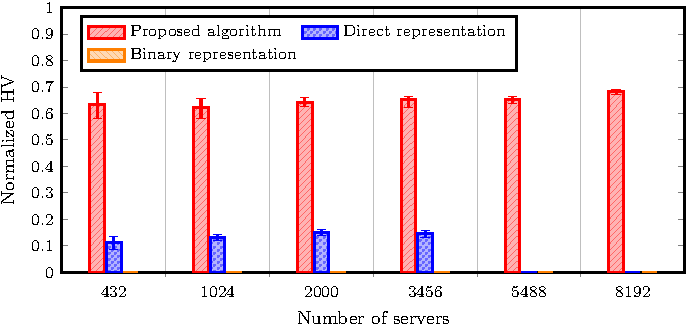
\includegraphics[width=\linewidth]{graphs/solution_representation/comparison-crop}
    \caption{Inter-quartile range of the HV when using different solution representations.}
    \label{fig:solution_representation_comparison}
\end{figure}
\begin{figure}[t!]
    \centering
    \begin{subfigure}[b]{0.49\linewidth}
        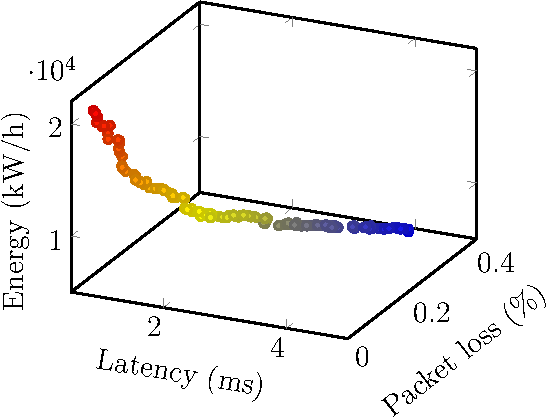
\includegraphics[width=\textwidth]{graphs/comparison/qm-crop}
        \caption{Proposed algorithm}
    \end{subfigure}
    \begin{subfigure}[b]{0.49\linewidth}
        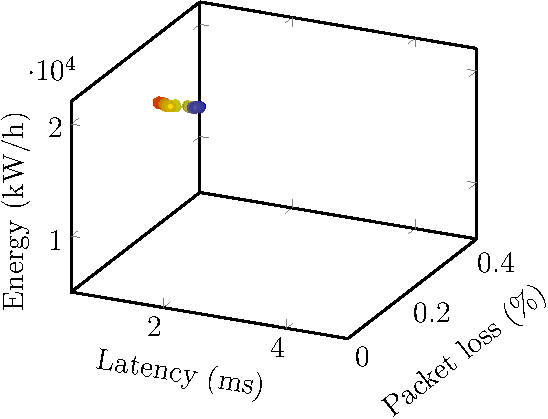
\includegraphics[width=\textwidth]{graphs/comparison/std-crop}
        \caption{Direct representation}
    \end{subfigure}

    \vspace{1em}
    \caption{Non-dominated front discovered when using different solution representations.}
    \label{fig:solution_representation_objectives}
\end{figure}

\textcolor{red}{
\subsubsection{Results}
From the results shown in Figs.~\ref{fig:solution_representation_comparison} and~\ref{fig:solution_representation_objectives}, we find that the solutions obtained by our proposed solution representation significantly outperform alternative representations. Our proposed solution representation has two advantages over existing representations. First, our proposed representation guarantees feasible solutions irregardless of the input. In contrast, both the direct and binary solution representations were unable to find feasible solutions to larger problem instances. Second, our proposed representation integrates domain knowledge to generate solutions with shorter average distances between VNFs causing the resultant solutions to be closer to the Pareto front than alternative representations. Existing solution representations do not utilize this information and instead rely solely on the optimization framework to locate high quality solutions.
}
\textcolor{red}{
Although the binary solution representation has been successfully applied to solve the VNFPP on small data centers (e.g.,~\cite{ChantreF20,KaurGK020,CharismiadisTPM20}), it does not scale well in the larger-scale problems considered in our experiments. With a binary solution representation, multiple VNFs to be placed on the same VM. This greatly complicates the search process compared to the direct or proposed solution representations with which this constraint is impossible to violate.
}
\textcolor{red}{
The direct solution representation is also only able to obtain feasible solutions to small data centers, as shown in~\pref{fig:solution_representation_objectives}, and exclusively finds solutions with high energy consumption. In particular, since a solution is only feasible when there is an instance of each VNF, solutions with more VNFs are more likely to be feasible than those with less VNFs and lower energy consumption. This leads the algorithm with the direct representation to be biased towards solutions with a high energy consumption. On larger problems with high numbers of VNFs, the direct solution representation is unable to find a solution with at least one instance of each VNF.
}

\vspace{0.5em}
\noindent
\framebox{\parbox{\dimexpr\linewidth-2\fboxsep-2\fboxrule}{
    \textcolor{red}{\textbf{\underline{Response to RQ4:}} \textit{The proposed solution representation allows the algorithm to discover significantly higher quality solutions than alternative solution representations.}}
    }}
    
\textcolor{red}{
\subsection{Comparison with Other Approaches}}
\label{sec:state_of_the_art}

\textcolor{red}{
\subsubsection{Methods}
To answer RQ5, we compare the performance of our tailored EMO algorithm with five state-of-the-art peer algorithms for solving VNFPPs. Specifically, the following two meta-heuristic algorithms use the NSGA-II as the baseline but use different genetic operators.
\begin{itemize}
    \item\underline{Binary representation}: In \cite{ChantreF20}, a string of binary digits are used to represent the placement of primary and secondary VNFs. To implement a fair comparison, we only consider the placement of the primary VNFs.
    \item\underline{Previous work}: We also compare our algorithm against our earlier work on this topic \cite{BillingsleyLMMG19}. This work utilized a direct representation with an earlier form of the tailored initialization operator.
\end{itemize}
The three heuristic algorithms are as follows.
\begin{itemize}
    \item\underline{BFDSU}~\cite{ZhangXLLGW17}: This is a modified best-fit decreasing heuristic that considers each VNF in turn and selects a server that can accommodate the VNF according to a predefined probability. In addition, the result is weighted towards selecting a server with a lower capacity.
    \item\underline{ESP-VDCE}~\cite{KaurGK020}: This is specifically designed for the Fat Tree data centers. It use a best fit approach but exclusively considers the servers nearest to where other VNFs of the same service have been placed.
    \item\underline{Stringer}~\cite{ChuaWZSH16}: This is also designed specifically for the Fat Tree data centers and it uses a round-robin placement strategy to place each VNF of each service in a sequence. The heuristic limits the available resources of each service and places a VNF on the first server with a sufficient capacity. If there is insufficient capacity in the data center for a VNF, the resources of each server are increased and the heuristic restarts from the first server.
\end{itemize}
Note that these heuristics assume that the number of service instances is known \textit{a priori}. Since each heuristic can only obtain a single solution, we generate a set of subproblems, each of which has a different number of service instances and is independently solved by a heuristic, to obtain a population of solutions at the end. In particular, we use the following two strategies to generate subproblems in our experiments.
\begin{itemize}
    \item One is to use the initialization operator developed in~\pref{sec:custom_operators} to serve our purpose. For the $i$th subproblem, the number of instances of the service $s$ is calculated as $N^I_{i,s}$ in~\pref{eq:num_services}.
    \item The other is to use the population obtained by our tailored EMO algorithm as a reference. For the $i$th subproblem, the number of instances of each service is the same as the $i$th solution obtained by our tailored EMO algorithm.
\end{itemize}
In our experiments, we generate $30$ VNFPP instances for six data centers with different sizes. To compare the performance of different algorithms, we use the QoS model developed in~\pref{sec:system_model} to evaluate the objective functions of the solutions obtained by different algorithms and use the HV indicator as the performance measure.
}
\textcolor{red}{
\subsubsection{Results}
}

\begin{figure*}[t!]
    \centering
    \begin{subfigure}[b]{0.19\linewidth}
        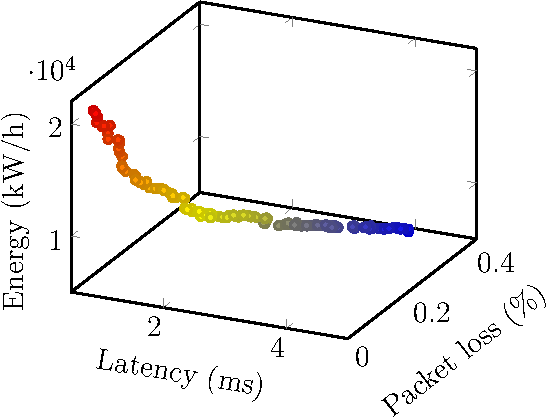
\includegraphics[width=\textwidth]{graphs/comparison/qm-crop}
        \caption{Proposed algorithm}
    \end{subfigure}
    \begin{subfigure}[b]{0.19\linewidth}
        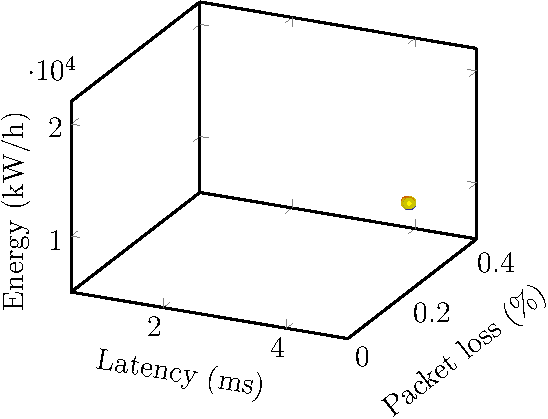
\includegraphics[width=\textwidth]{graphs/comparison/previous-crop}
        \caption{Previous algorithm}
    \end{subfigure}
    \begin{subfigure}[b]{0.19\linewidth}
        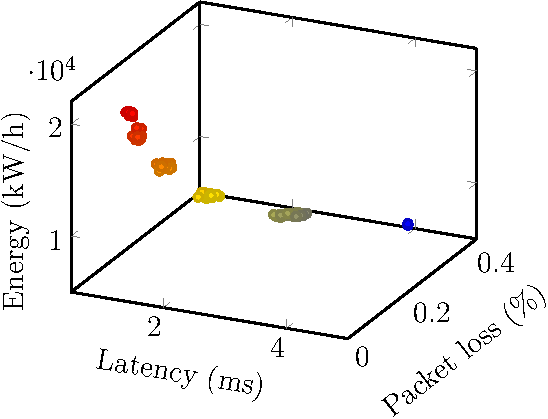
\includegraphics[width=\textwidth]{graphs/comparison/esp_vdce-crop}
        \caption{ESP-VDCE \cite{KaurGK020}}
    \end{subfigure}
    \begin{subfigure}[b]{0.19\linewidth}
        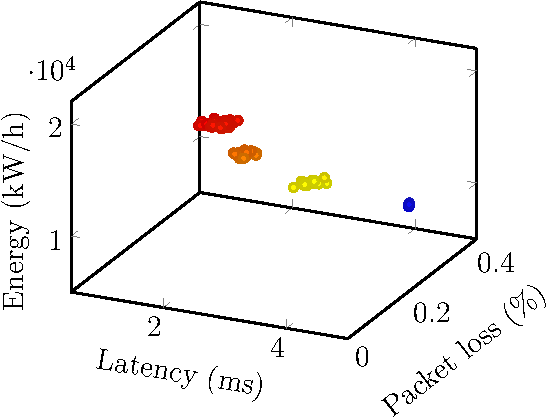
\includegraphics[width=\textwidth]{graphs/comparison/bfdsu-crop}
        \caption{BFDSU \cite{ZhangXLLGW17}}
    \end{subfigure}
    \begin{subfigure}[b]{0.19\linewidth}
        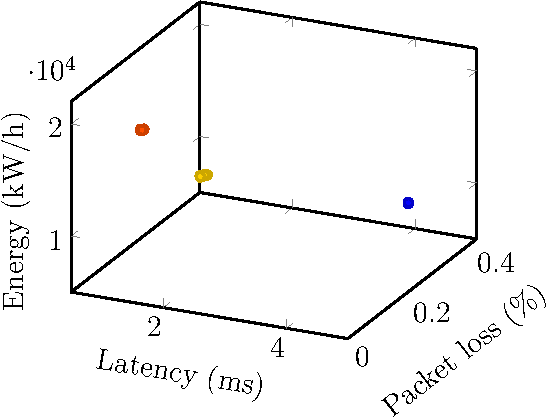
\includegraphics[width=\textwidth]{graphs/comparison/stringer-crop}
        \caption{Stringer \cite{ChuaWZSH16}}
    \end{subfigure}

    \vspace{1em}
    \caption{Non-dominated front found by five algorithms. Subproblems for the heuristic algorithms were generated using our proposed initialization operator. The binary solution representation is omitted as it resulted in no feasible solution at all.}
    \label{fig:alg_objectives}
\end{figure*}

\begin{figure*}
    \centering
    \hfill
    \begin{minipage}[t]{.48\textwidth}
        \centering
        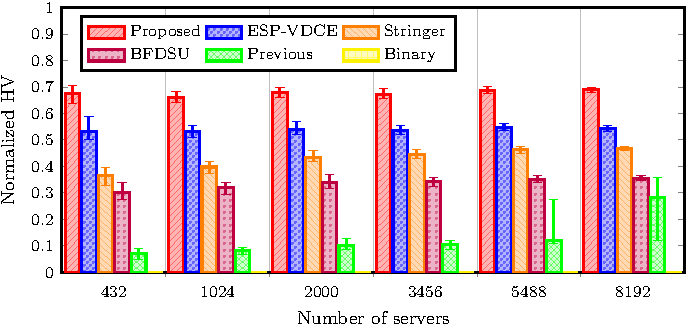
\includegraphics[width=\columnwidth]{graphs/comparison/comparison-crop}
        \caption{Inter-quartile range of the HV when using the initialization operator to generate subproblems for the heuristic algorithms.}
        \label{fig:alg_comparison}
    \end{minipage}\hfill
    \begin{minipage}[t]{.48\textwidth}
        \centering
        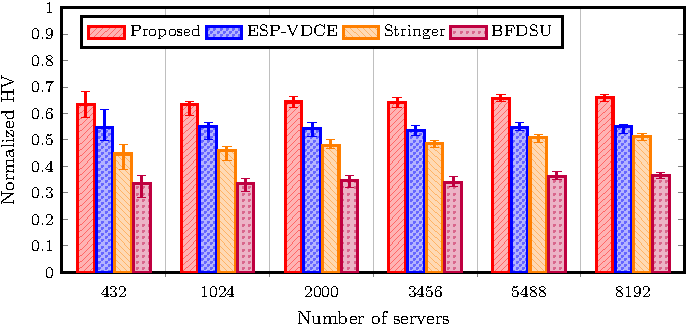
\includegraphics[width=\columnwidth]{graphs/comparison/alg_fixed-crop}
        \caption{Inter-quartile range of the HV when using the solutions of our proposed algorithm to generate subproblems for the heuristic algorithms.}
        \label{fig:alg_fixed}
    \end{minipage}
    \hfill
\end{figure*}

\textcolor{red}{
From the results shown in~\pref{fig:alg_comparison} and~\pref{fig:alg_fixed}, it is clear that our proposed algorithm outperforms other competitors on all test cases. This can be attributed to our two proposed operators. First, it is clear from \pref{fig:alg_objectives} that proposed operators enable a diverse population of solutions. Our two proposed operators work together towards this goal. The initialization operator produces a diverse range of possible solutions, whilst the solution representation ensures that these solutions are feasible.
}

\textcolor{red}{
Second, our proposed solution representation minimizes the distance between sequential VNFs, improving the overall QoS. We note that the two best performing algorithms, our proposed algorithm and ESP-VDCE, aim to minimize the distance between sequential VNFs. In contrast, both BFDSU and Stringer tend to produce longer path lengths thus lead to significantly worse solutions than our proposed algorithm. Since Stringer restricts the capacity of each server, it causes services to be placed across multiple servers. Likewise, the stochastic component of BFDSU can cause it to place VNFs far away from any other VNF of the service. In contrast, our proposed algorithm incorporates useful information into the optimization process and places sequential VNFs close by thus leading to better solutions.
}

\textcolor{red}{
A final benefit of our algorithm is that it can iteratively improve the placements to minimize the energy consumption and QoS. Although ESP-VDCE does consider the path length, it otherwise uses a simple first fit heuristic that cannot consider how service instances should be placed in relation to each other. As a consequence, the performance of ESP-VDCE depends on the order in which services are considered. Our proposed algorithm considers the problem holistically and can make informed placement decisions.
}

\vspace{1em}
\noindent
\framebox{\parbox{\dimexpr\linewidth-2\fboxsep-2\fboxrule}{
        \textcolor{red}{\textbf{\underline{Response to RQ5:}} \textit{Our proposed tailored EMO algorithm obtains significantly better solutions in terms of both convergence and diversity compared to other state-of-the-art peer algorithms.}}
    }}

\subsection{Effectiveness on Constraint Handling}
\label{sec:custom_operators}

\subsubsection{Methods}

RQ6 aims to validate the effectiveness of our proposed solution representation for handling challenging anti-affinity and limited licenses constraints. We generated $30$ problem instances for a small data center with $412$ servers\footnote{Only the small data center is considered here in view of the poor scalability of the direct representation reported in~\pref{sec:state_of_the_art}.}. Note that we only compare our proposed algorithm with the meta-heuristic approach with the direct solution representation in our experiments given the poor performance of the binary solution representation reported in~\pref{sec:state_of_the_art} and the inability of the heuristic approaches to solve constrained VNFPPs.

For the anti-affinity constraints, we considered different numbers of anti-affinity services and similarly, for the limited licenses constraints we considered different numbers of limited license VNFs and different numbers of licenses for each VNF. Since different VNFs have different service rates, we calculate the expected maximum number of instances of each VNF that could be accommodated by the data center (i.e. the maximum value of $N^I$ in the \pref{eq:num_services}) and restrict the solution to use a fraction of this number of licenses.

\subsubsection{Results}
From the results shown in Figs.~\ref{fig:anti_affinity} and \ref{fig:limited_licenses}, it is clear to see that the direct representation cannot find any feasible solution due to the narrow feasible search space. In contrast, our proposed operators are still able to find a diverse set of feasible solutions even for these highly constrained problems. As shown in \pref{fig:anti_affinity}, our algorithm produces consistently good results on the anti-affinity problems. This is a benefit of our proposed solution representation which ensures the satisfaction of the anti-affinity constraints. Since the solutions are guaranteed to be feasible, the algorithm should only optimize the number and placement of service instances. Any degradation in the HV indicator can be attributed to the narrower feasible search space causing better alternatives to be infeasible. In particular, anti-affinity constraints prevent VNFs of other services from being placed on a server thus can prevents a server from being fully utilized.

According to our empirical results, the limited licenses constraints appear to be more challenging. As shown in~\pref{fig:limited_licenses}, populations obtained by our proposed algorithm have a better HV value when a large number of licenses is allowed, whereas it falls down when fewer licenses are available. Furthermore, the percentage of VNFs that are affected has little impact. The lower HV values can be explained by a loss of diversity as a result of the feasible solution space being constrained. If any VNF in a service is constrained by a limited license constraint, this limits the number of service instances that can be placed. Hence the percentage of VNFs that can be placed is less significant as it is likely that a VNF in the service is already constrained.

\vspace{1em}
\noindent
\framebox{\parbox{\dimexpr\linewidth-2\fboxsep-2\fboxrule}{
        \textbf{\underline{Response to RQ6:}} \textit{From our empirical results, we find that our proposed genotype-phenotype solution representation is superior for handling highly constrained VNFPP.}
    }}

\begin{figure}[t!]
    \centering
    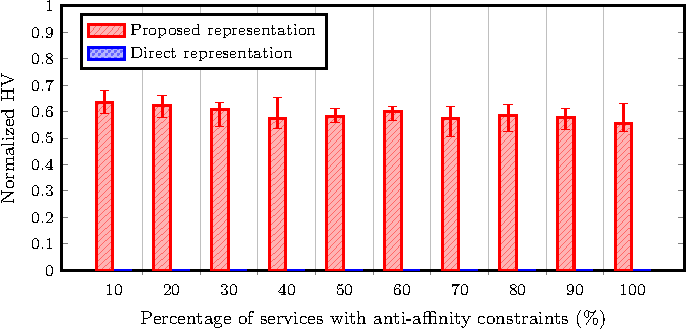
\includegraphics[width=\linewidth]{graphs/constraints/anti_affinity-crop}
    \caption{Inter-quartile range of the HV for different solution representations and anti-affinity constraints.}
    \label{fig:anti_affinity}
\end{figure}
\begin{figure}[t!]
    \centering
    \begin{subfigure}[b]{0.48\linewidth}
        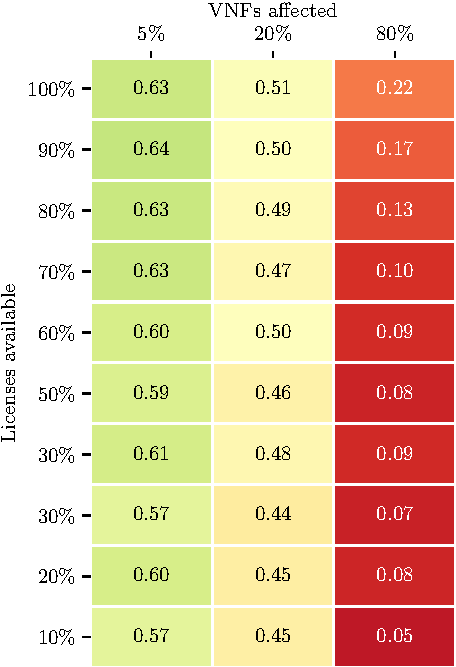
\includegraphics[width=\textwidth]{graphs/constraints/ca_NSGAII_LIM-crop}
        \caption{Proposed representation}
    \end{subfigure}
    \vspace{1em}
    \begin{subfigure}[b]{0.3732\linewidth}
        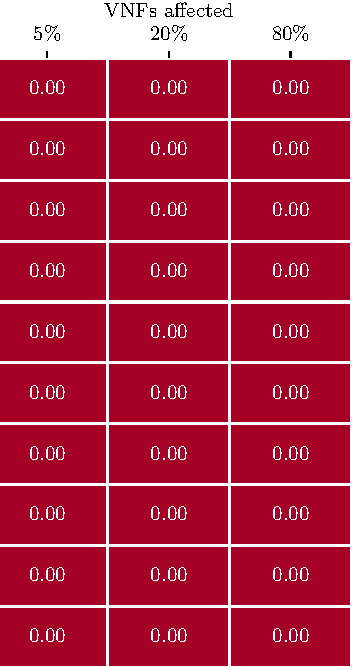
\includegraphics[width=\textwidth]{graphs/constraints/std_NSGAII_LIM-crop}
        \caption{Direct representation}
    \end{subfigure}
    \vspace{0.3em}

    \hspace{2em}
    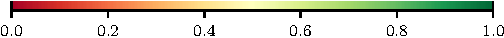
\includegraphics[width=.8\linewidth]{graphs/constraints/key-crop}
    \caption{Mean normalized HV under max license constraints.}
    \label{fig:limited_licenses}
\end{figure}


% ~ 1 page
% !TeX root = ./main.tex

\section{Conclusion}
\label{sec:conclusion}

% Single opening sentence then re-Enumerate principle contributions
By utilizing data center resources efficiently, we can provide high quality services and minimize their environmental impact. This work provided an efficient and accurate analytical model with which to evaluate the QoS of large data centers. To solve our VNFPP, we proposed a problem specific solution representation along with a tailored initialization strategy to guarantee the generation of feasible solutions, both of which are directly pluggable into any EMO algorithm. There are four main findings from our comprehensive experiments.
\begin{itemize}
    \item Our proposed model is significantly more accurate than the existing competitors, especially when data center components become self-dependent.
    \item Widely used surrogate models provide insufficient information to produce diverse solutions when being used to solve our VNFPP. In contrast, accurate models that consider packet loss are effective.
    \item Our proposed algorithm produces significantly better solutions than its competitors, especially when solving large scale VNFPPs.% In particular, our algorithm provides superior results over existing heuristic algorithms, which do not consider how the placement of services can affect each other, and also against alternative meta-heuristic algorithms which use less suitable solution representations.  % 'Better' or 'more diverse / optimal' ?
    \item Our proposed solution representation is highly effective for challenging constraints. In contrast, alternative solution representations fail to find feasible solutions.
\end{itemize}

% Enumerate future extensions
\textcolor{red}{
There are some disadvantages and extensions to our current approach that could be considered in future work.
\begin{itemize}
    \item A limitation of our proposed algorithm is that it is only applicable to Fat Tree network topologies. However, the underlying heuristic of our work - prefer to place VNFs on nearby servers - is applicable to any data center. It would be interesting to extend this work to arbitrary topologies.
    \item Although execution time is not a priority in this work, it is notable that metaheuristic approaches are typically slower than heuristic algorithms since they requires a large number of model evaluations. That said, the significant improvements we make over existing heuristic alternatives justifies our approach. In future work, fast heuristic alternatives to accurate models may reduce this gap between heuristic and metaheuristic algorithms.
    \item Furthermore, there are interesting possibilities in exploring the impact of different types of VNF and service. It would be interesting to determine how an alternative problem formulation would affect the design and results of a meta-heuristic alternative.
\end{itemize}
}

\section*{Acknowledgment}
K. Li was supported by UKRI Future Leaders Fellowship (Grant No. MR/S017062/1) and Amazon Research Awards. J. Billingsley was supported by EPSRC Industrial CASE and British Telecom (Grant No. 16000177).

\bibliographystyle{IEEEtran}
\bibliography{IEEEabrv,bibliography}

\end{document}
